% Incluyendo el preambulo de LaTeX para configurar los paquetes que se vayan usando
% Configuracion inicial del documento
\documentclass[a4paper]{article}

% Paquetes utilizados
\usepackage[utf8]{inputenc}
\usepackage[spanish, es-tabla]{babel}
\usepackage{float}
\usepackage{graphicx}
\usepackage{multirow}
\usepackage{circuitikz}

% Paquetes de matematica
\usepackage{amsmath}
\usepackage{amssymb}
\usepackage{steinmetz}

% Paquetes para excel
\usepackage{csvsimple}

% Configuracion del informe
\setlength{\parindent}{0pt}
\setcounter{secnumdepth}{0}

\usepackage[a4paper, 
    includehead, 
    footskip=7mm, 
    headsep=6mm, 
    headheight=4.8mm,
    top=25mm, bottom=25mm, left=25mm, right=25mm]{geometry}

\usepackage{hyperref}
\hypersetup{
    colorlinks=true,
    linkcolor=blue,
    filecolor=magenta,      
    urlcolor=blue,
    citecolor=blue,    
}

% Abrir y crear el documento, llamar a cada uno de los ejercicios
\begin{document}

    % Crear y configurar el titulo/caratula del informe
    \title{
        \normalfont \normalsize \textsc{Instituto Tecnol\'ogico de Buenos Aires} \\ [25pt]
        \huge Trabajo Pr\'actico Nº 3 \\
        \author{
            \\Grupo 1:\\\\Galdeman, Agust\'in Ignacio\\Gaytan, Joaqu\'in Oscar\\Kammann, Lucas Agust\'in\\Maselli, Carlos Javier\\ \\ \\ \\
            Profesores: \\\\ Cossutta, Pablo Mart\'in\\Weill, Mar\'ia Alejandra\\Salvati, Mat\'ias Dami\'an \\ \\ \\ 
        } 
        \text{Laboratorio de Electr\'onica - 2019}
    }
    \pagenumbering{arabic}

    \maketitle
    \newpage

    % Crear indice del informe
    \tableofcontents

    % Incluyendo los ejercicios realizados
    \newpage
    \section{Introducci\'on}

En este informe se armarán, analizarán y medirán circuitos RC simples de primer orden con el objetivo de familizarizarse con el set de instrumentos provistos por el laboratorio. Se hará especial énfasis en la correcta utilización del osciloscopio y en lo que implica medir un circuito. Finalmente, se desarrollarán dos experiemntos para comprender mejor el funcionamiento del osciloscopio y los distintos sistemas que lo componen.
    \newpage
    


\section{Caracterizaci\'on de componentes pasivos}
En esta secci\'on se analiza el comportamiento de los componentes pasivos en funci\'on de la frecuencia de operaci\'on, en particular de un capacitor y un inductor.
Para dicho an\'alisis se realiza un barrido en frecuencias desde $10Hz$ a $10MHz$.

\subsection{Medici\'on del capacitor}
Para la medici\'on se utiliza un capacitor de $22nF$ de film y se configura el analizador de impedancias en modelo paralelo para medir fase y admitancia. En este caso, debido a las caracter\'isticas particulares del componente, no es posible realizar el barrido de frecuencias completo.
\subsubsection{Resultados}
Se muestran en la Tabla \ref{tab:Med_CAP}  los resultados obtenidos de las mediciones y en la Figura \ref{fig:Med_CAP} los respectivos  gr\'aficos realizados a partir de estas.

\begin{table}[H]
    \centering
    \resizebox{0.5\textwidth}{!}{%
        \begin{tabular}{ccccc}
            \hline
            \begin{tabular}[c]{@{}c@{}}Frecuencia\\   (Hz)\end{tabular} & Capacidad (F) & \begin{tabular}[c]{@{}c@{}}Factor de\\   disipación\end{tabular} & Admitancia (s) & Fase ($^\circ$) \\ \hline
            5 & 2.20E-08 & 0.006 & 6.80E-07 & 89.5 \\
            10 & 2.19E-08 & 0.006 & 1.38E-06 & 89.9 \\
            20 & 2.20E-08 & 0 & 2.76E-06 & 90 \\
            100 & 2.19E-08 & 0.0012 & 1.38E-05 & 89.93 \\
            300 & 2.19E-08 & 0.0025 & 4.13E-05 & 89.86 \\
            1000 & 2.19E-08 & 0.0039 & 1.37E-04 & 89.78 \\
            3000 & 2.18E-08 & 0.0064 & 4.10E-04 & 89.64 \\
            10000 & 2.17E-08 & 0.0086 & 1.36E-03 & 89.51 \\
            30000 & 2.15E-08 & 0.0124 & 4.05E-03 & 89.29 \\
            80000 & 2.13E-08 & 0.0157 & 1.07E-02 & 89.1 \\
            100000 & 2.13E-08 & 0.0165 & 1.34E-02 & 89.06 \\
            150000 & 2.12E-08 & 0.018 & 2.00E-02 & 88.97 \\
            200000 & 2.11E-08 & 0.0191 & 2.66E-02 & 88.91 \\
            300000 & 2.11E-08 & 0.0211 & 3.97E-02 & 88.79 \\
            400000 & 2.10E-08 & 0.0228 & 5.28E-02 & 88.69 \\
            500000 & 2.10E-08 & 0.0245 & 6.60E-02 & 88.6 \\
            600000 & 2.10E-08 & 0.0262 & 7.91E-02 & 88.5 \\
            700000 & 2.10E-08 & 0.0279 & 9.24E-02 & 88.4 \\
            750000 & 2.10E-08 & 0.0287 & 9.90E-02 & 88.35 \\
            780000 & 2.10E-08 & 0.0292 & 1.03E-01 & 88.32 \\
            800000 & 2.10E-08 & 0.0296 & 1.06E-01 & 88.31 \\
            825000 & 2.10E-08 & 0.03 & 1.09E-01 & 88.28 \\
            850000 & 2.10E-08 & 0.0305 & 1.12E-01 & 88.25 \\
            900000 & 2.11E-08 & 0.0313 & 1.19E-01 & 88.18 \\
            1000000 & 2.11E-08 & 0.033 & 0.133 & 88.1 \\
            2000000 & 2.19E-08 & 0.052 & 0.276 & 87 \\
            3000000 & 2.36E-08 & 0.077 & 0.447 & 85.6 \\
            4000000 & 2.66E-08 & 0.112 & 0.673 & 83.6 \\
            5000000 & 3.18E-08 & 0.166 & 1.012 & 80.6 \\
             \hline
        \end{tabular}%
    }
    \caption{Mediciones del capacitor}
    \label{tab:Med_CAP}
\end{table}

\begin{figure}[H]
    \centering
    \resizebox{\textwidth}{!}{
        \begin{tabular}{c c}
            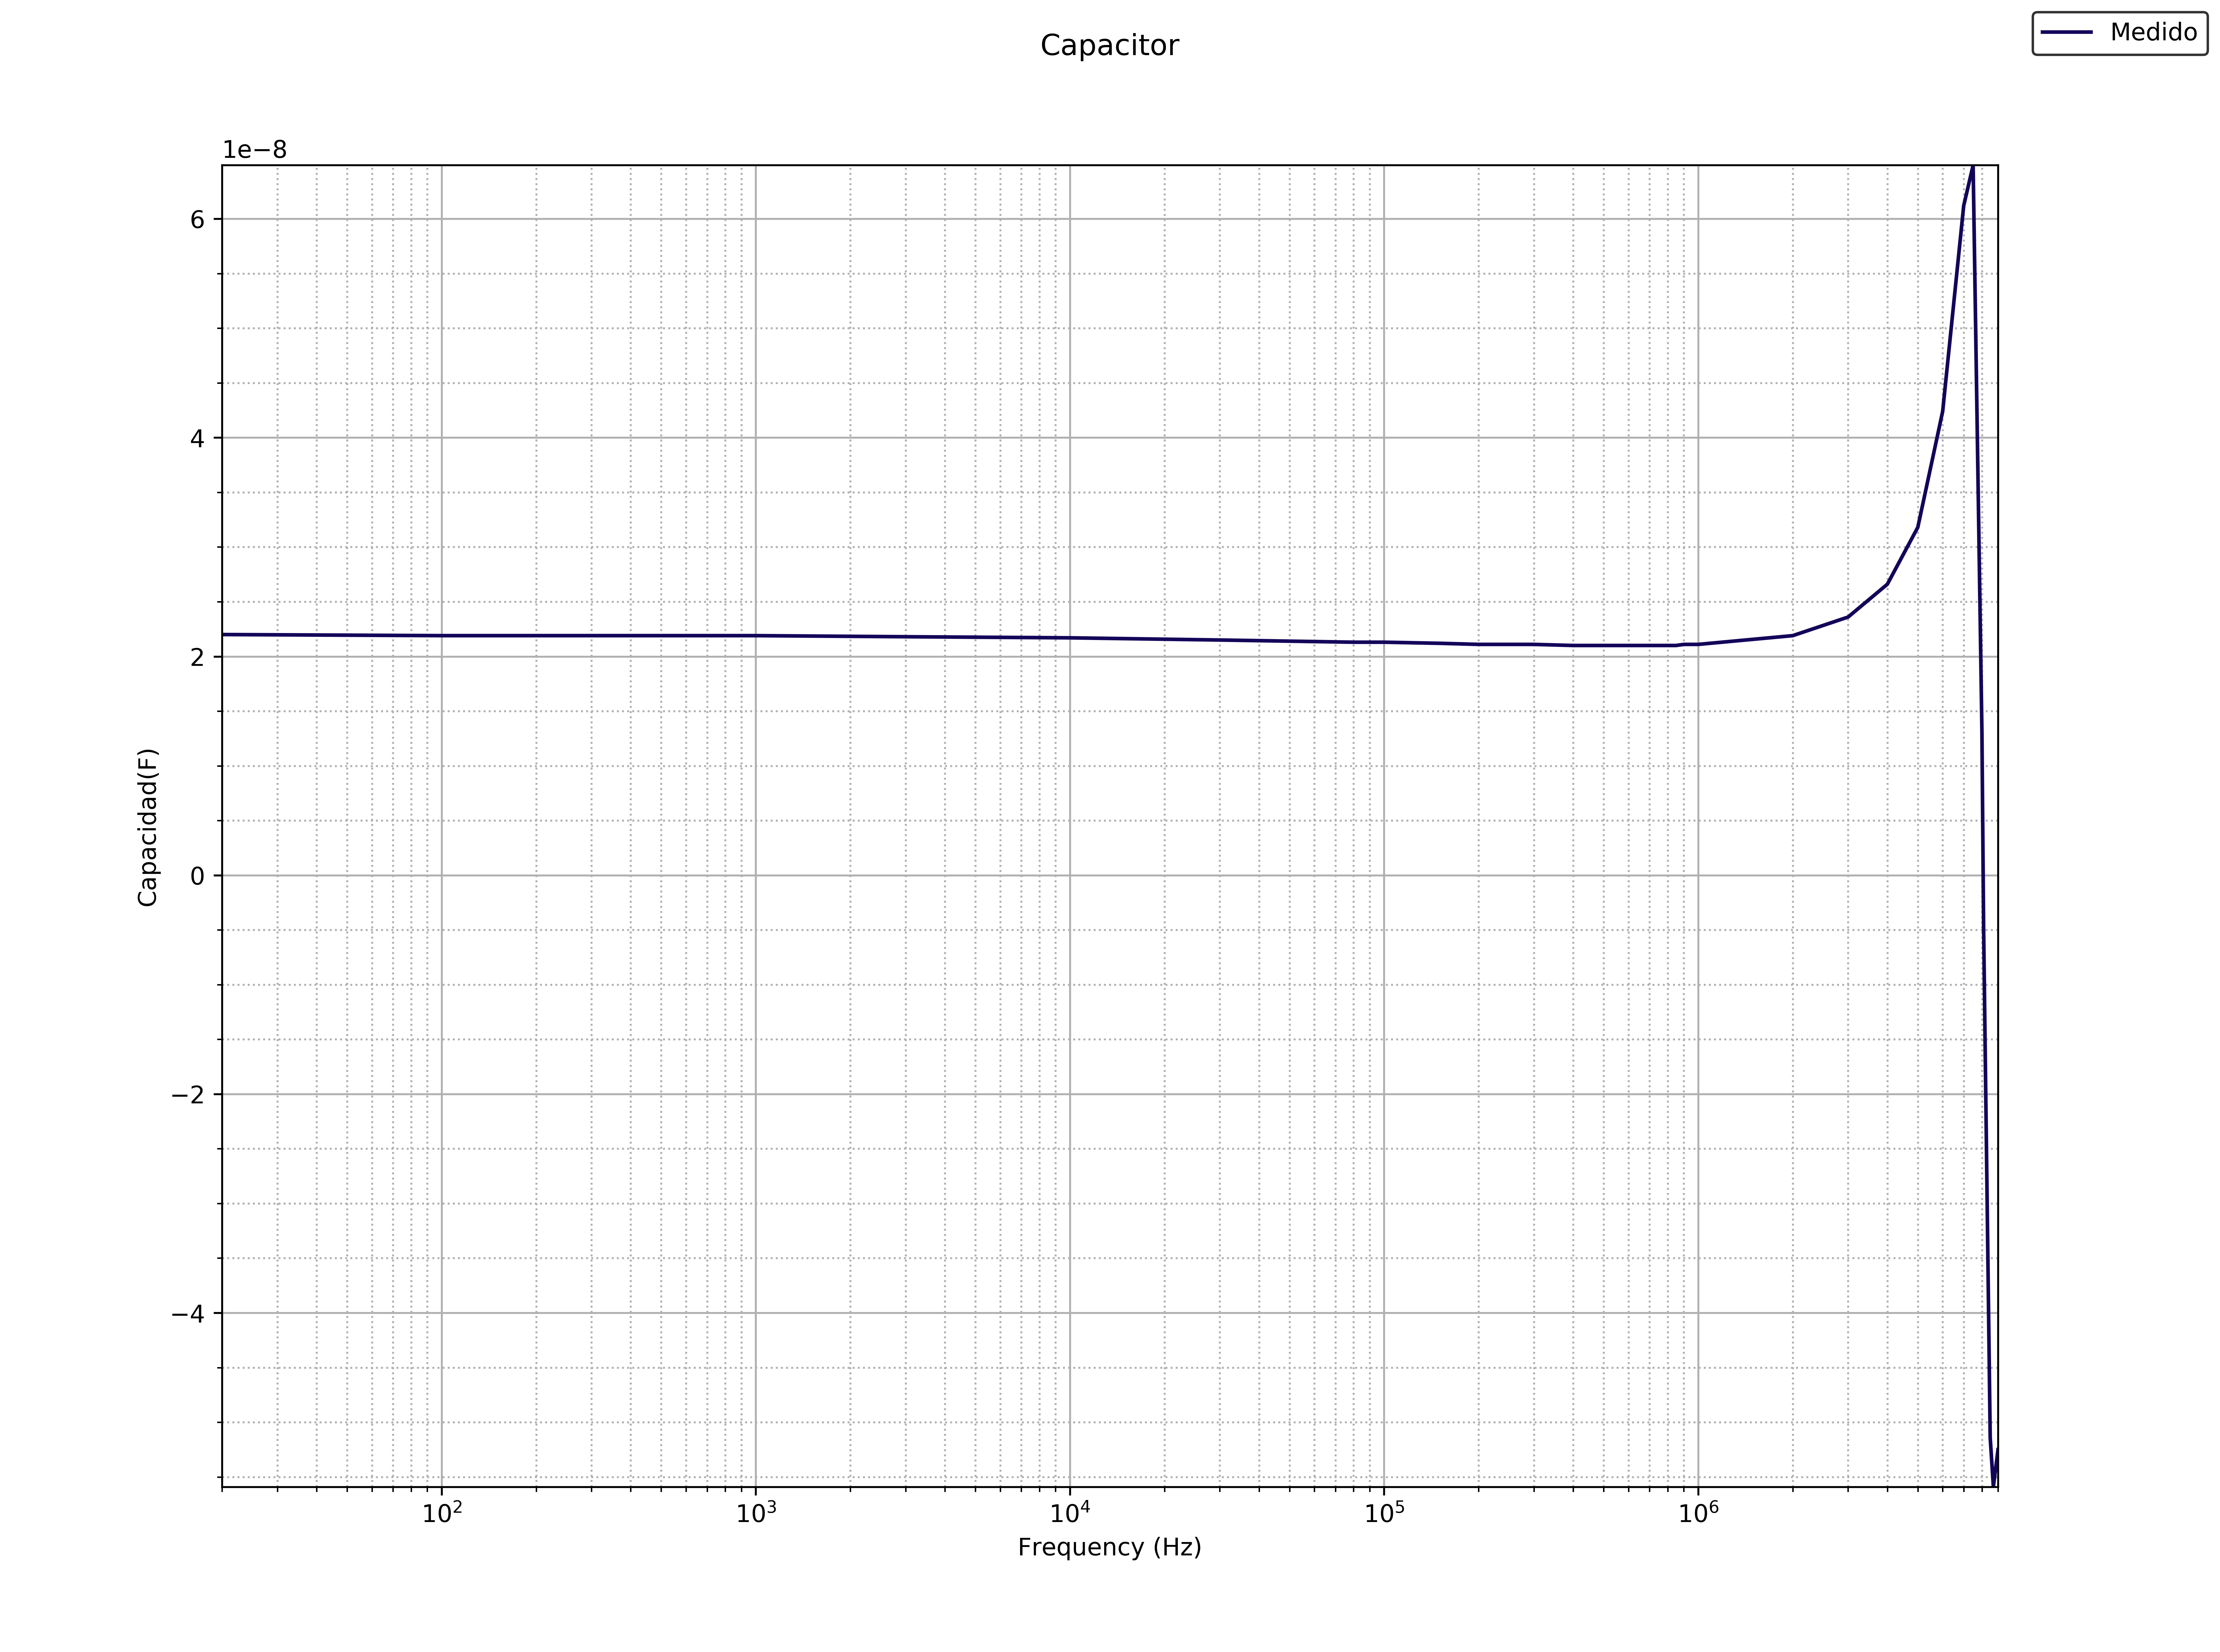
\includegraphics{Recursos/capacidad_medida.png}&
            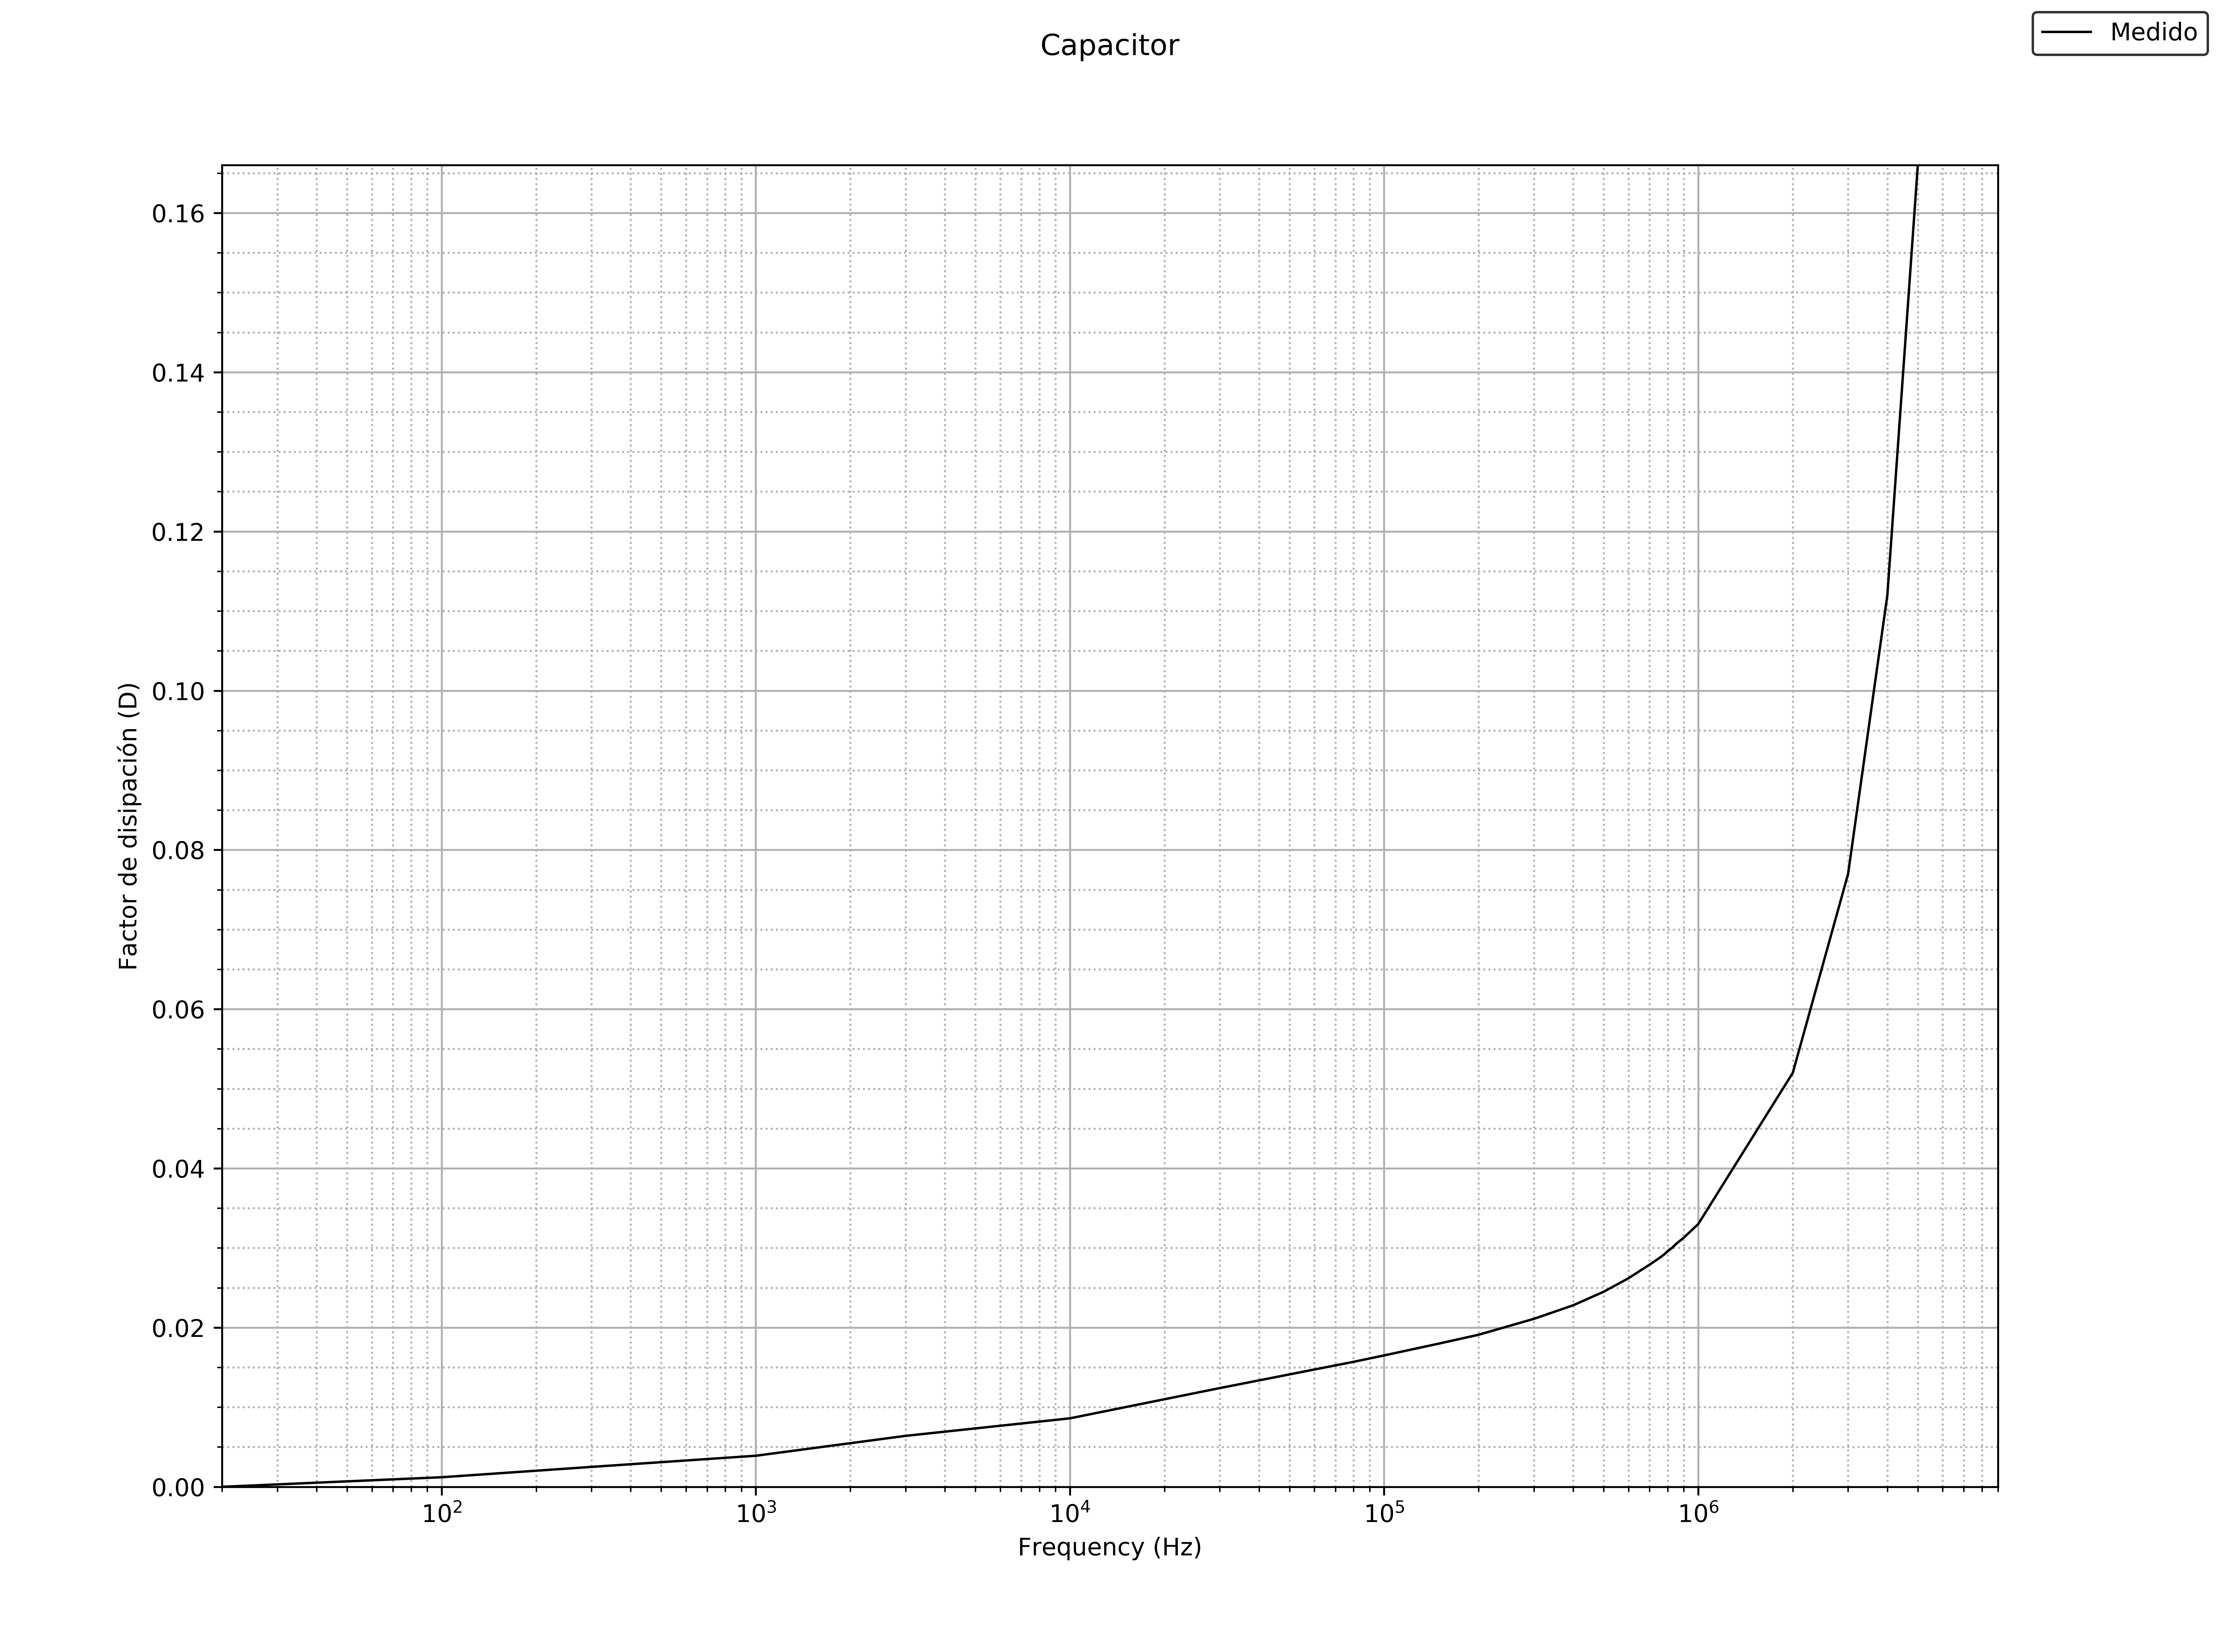
\includegraphics{Recursos/perdidas_medida_cap.png} \\
            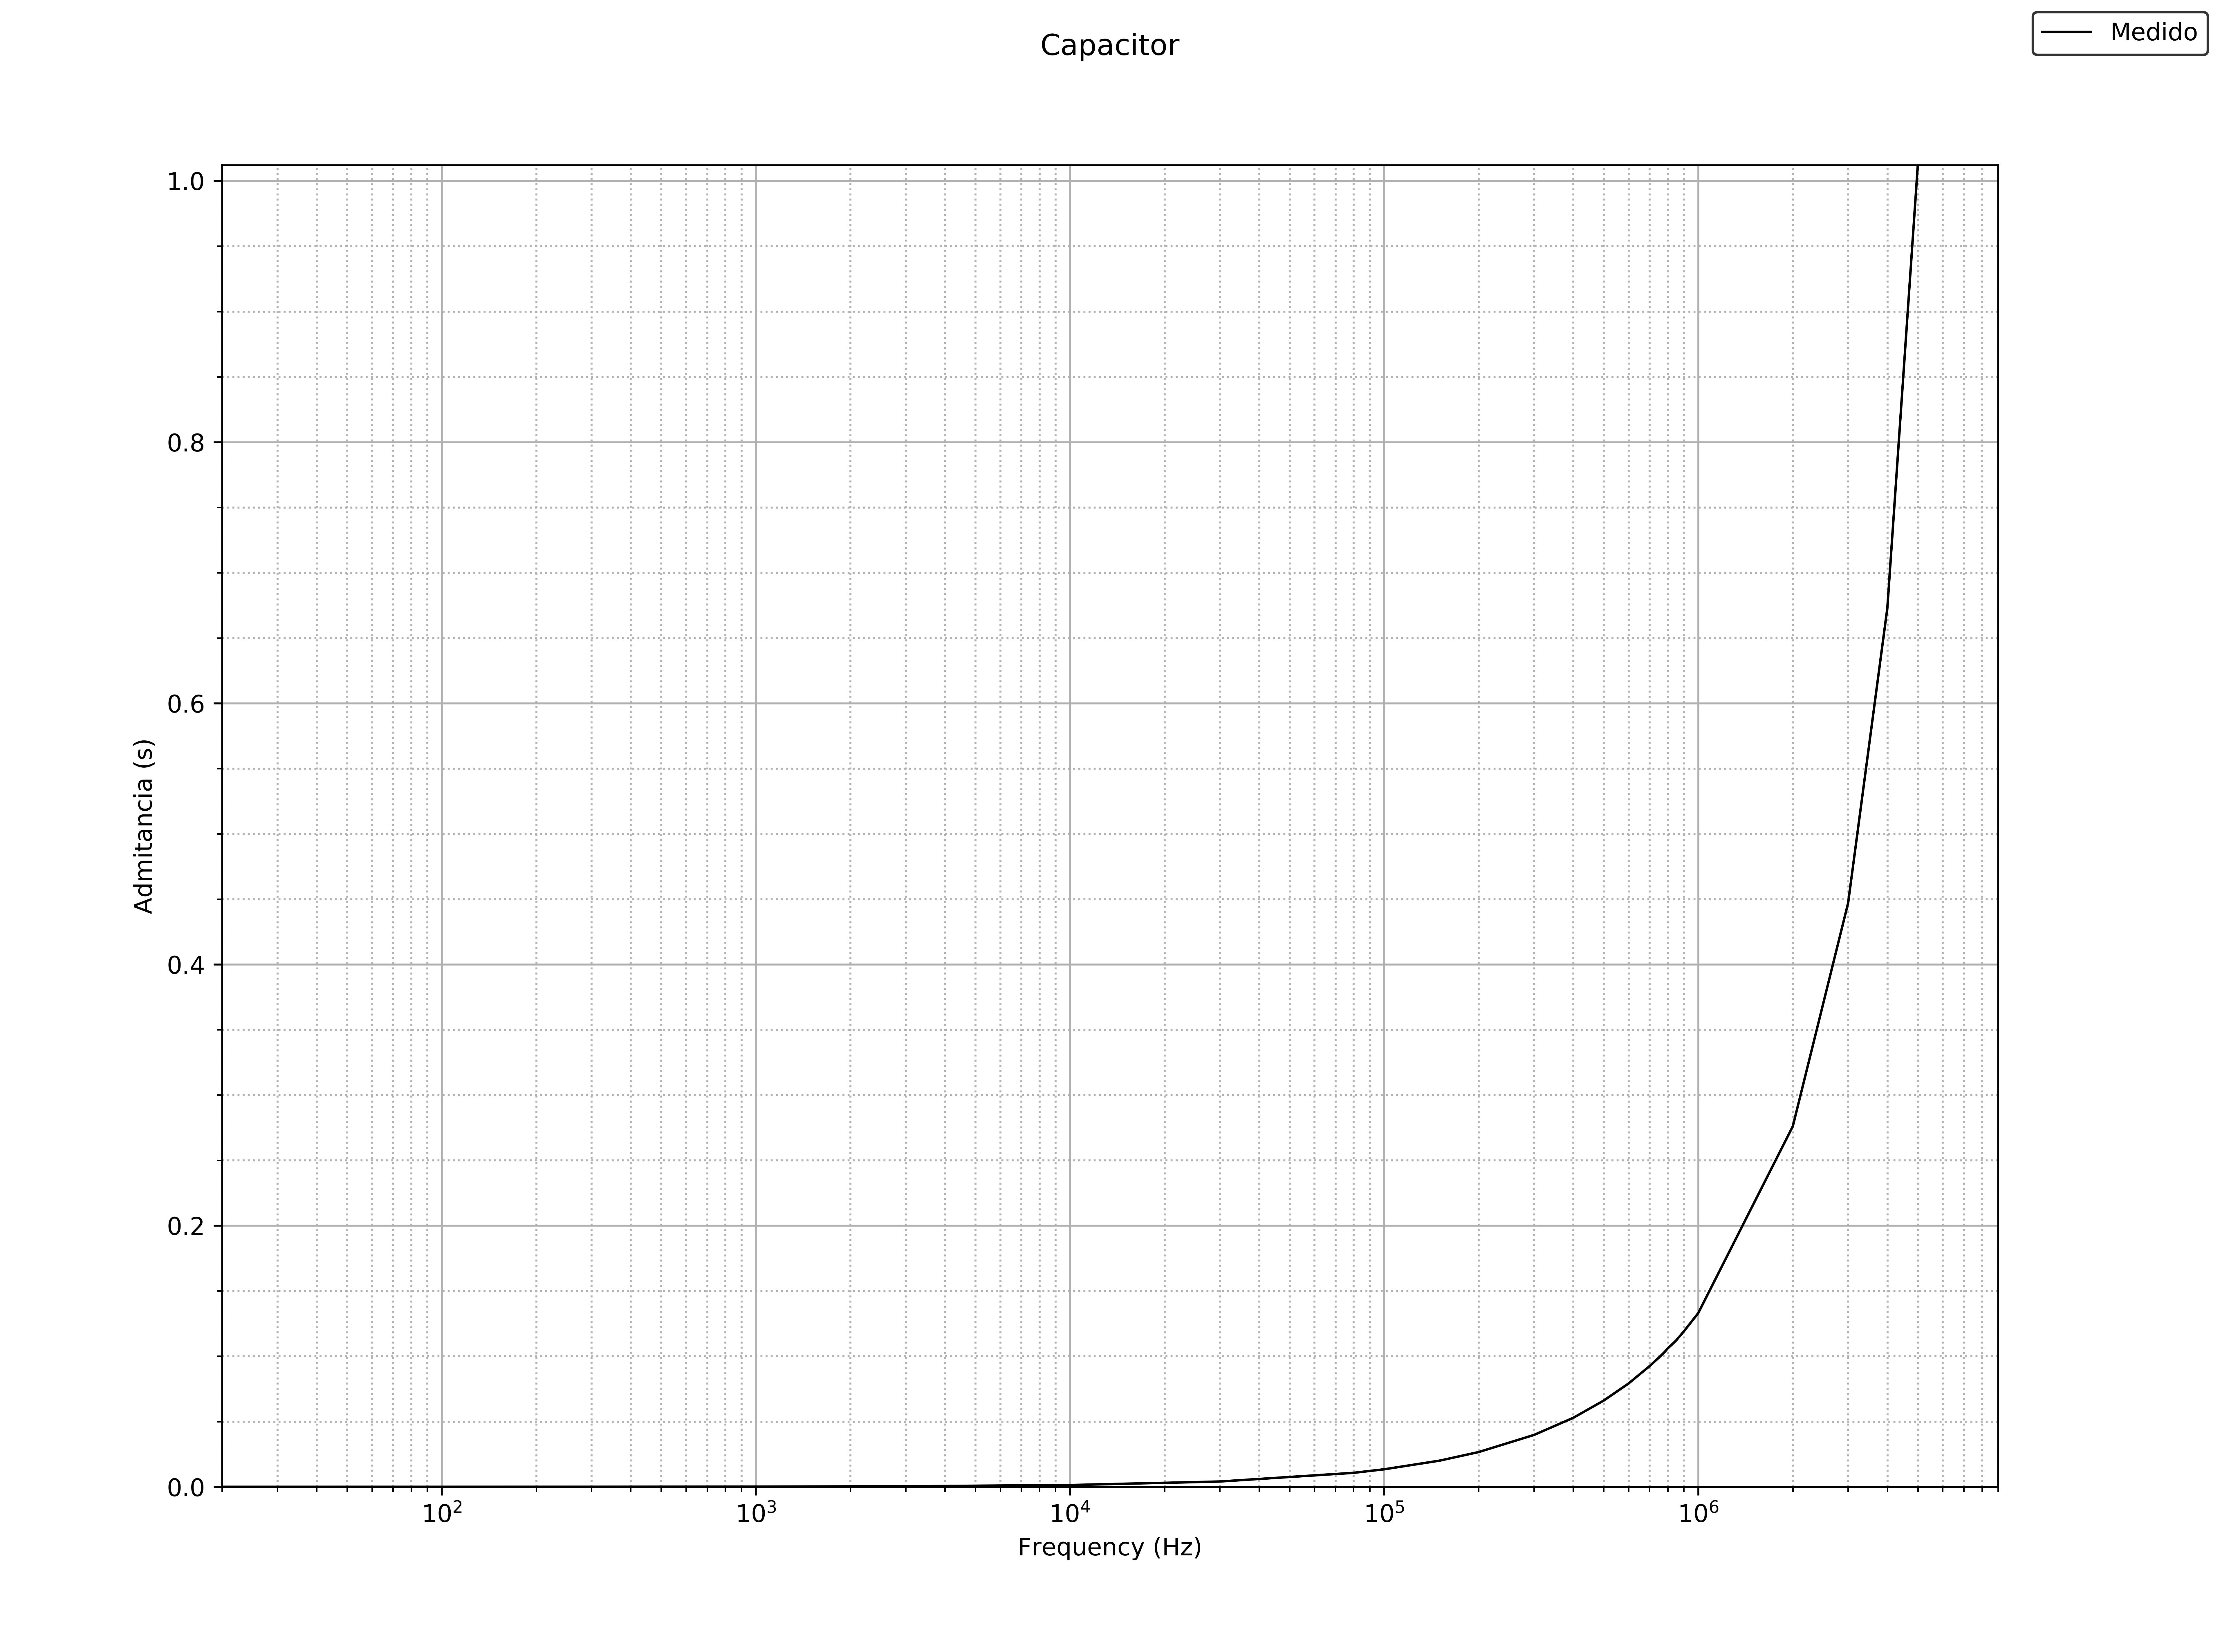
\includegraphics{Recursos/admitancia_medida_cap.png} &
            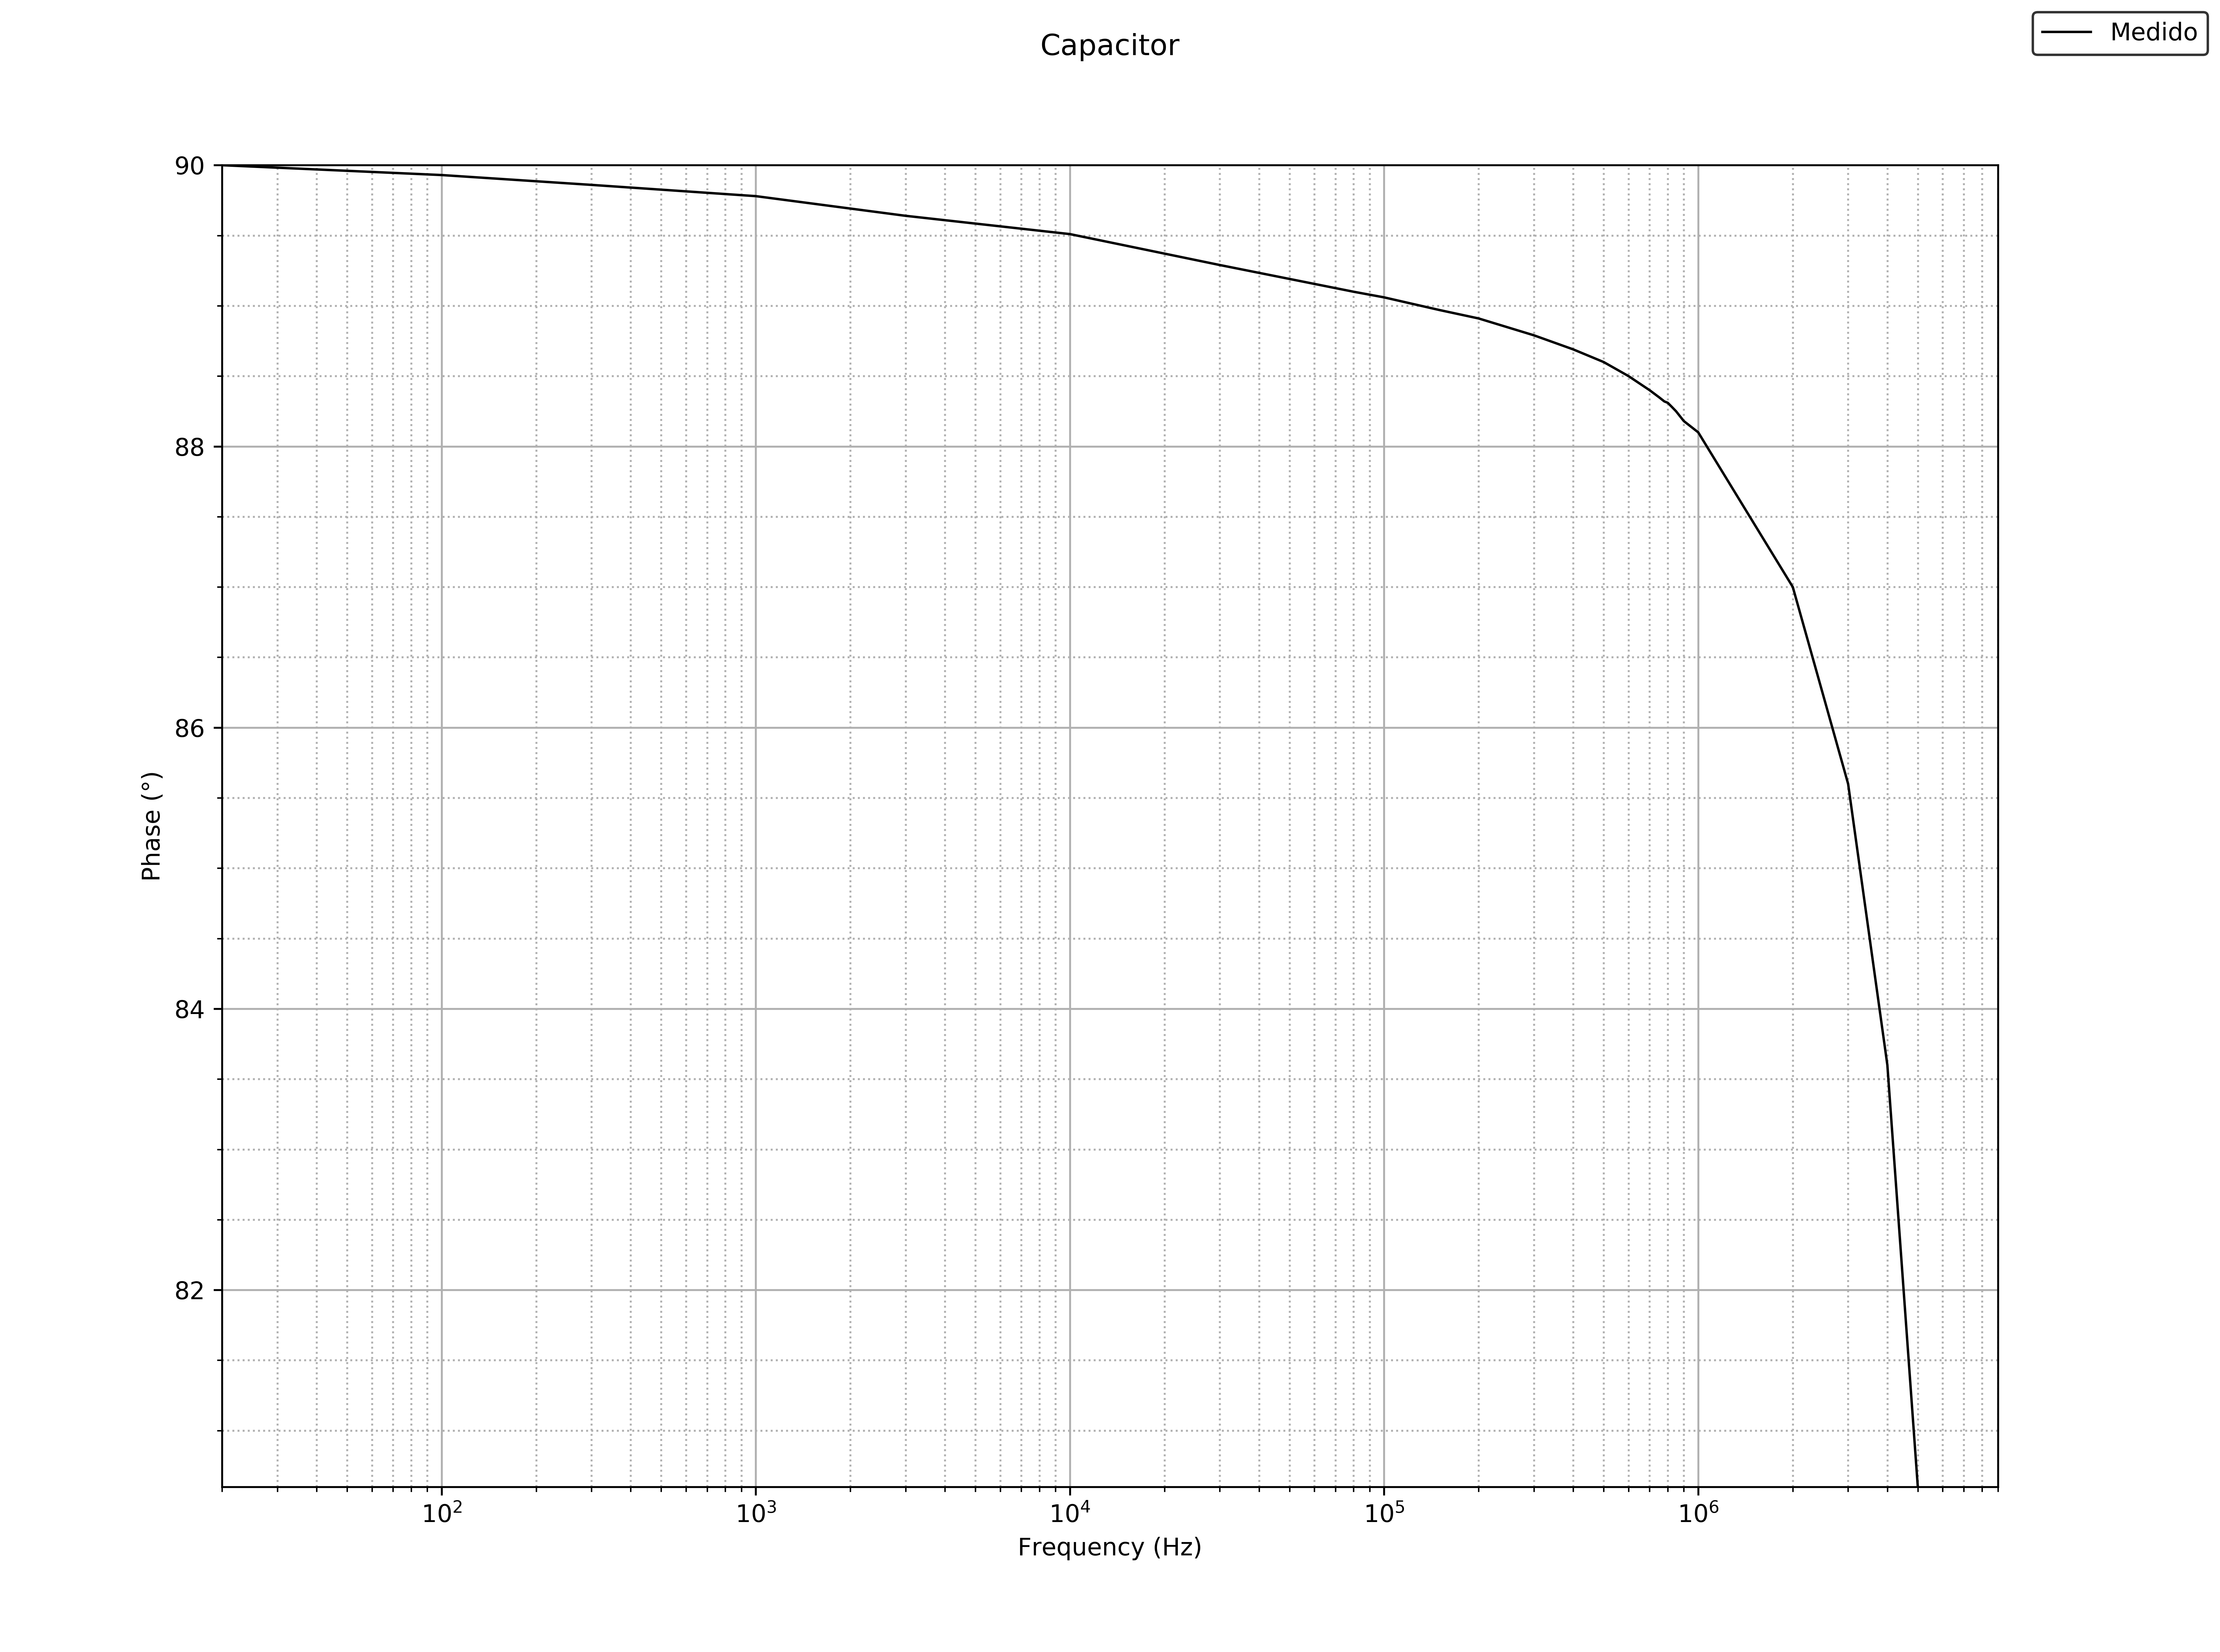
\includegraphics{Recursos/fase_medida_cap.png}

        \end{tabular}
    }
    \caption{Gr\'aficos realizados a partir de las mediciones}
    \label{fig:Med_CAP}
    
\end{figure}    


\subsubsection{Modelizaci\'on del comportamiento observado}
Se propone el circuito de la Figura \ref{fig:modelo_CAP} con el fin de encontrar un modelo que se ajuste al comportamiento real del capacitor tanto en impedancia como en fase.
\begin{figure}[H]
    \centering
    \resizebox{0.5\textwidth}{!}{
        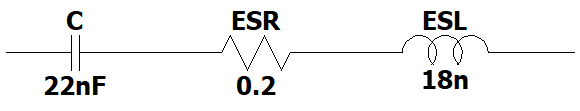
\includegraphics{Recursos/Modelo_cap.png}
    }
    \caption{Modelo de comportamiento del capacitor}
    \label{fig:modelo_CAP}
\end{figure}
El valor de la inductancia se parte de que la frecuencia de corte del sistema se encuentra en el punto donde el valor de capacidad arrojado por el analizador de impedancias pase de ser positivo a negativo, es decir, cuando el capacitor comienza a comportarse como un inductor. Del las mediciones se obtiene $f_{0} = 8MHz$. Luego, utilizando las f\'ormulas conocidas para un RLC serie mostradas en \ref{eq:RLC_CAP} y asumiendo que el valor de C es el nominal del componente utilizado.
\begin{equation}
    \omega_0 = \frac{1}{\sqrt{L \cdot C}} = 2 \cdot \pi \cdot f_0
    \label{eq:RLC_CAP}
\end{equation}
Resolviendo \ref{eq:RLC_CAP} se obtiene $L = 18nHy$.
Para ESR, se busca un valor iterando repetidas veces, hasta obtener una curva que se aproxime a la medida para la admitancia del capacitor.

Se muestran en la Figura \ref{fig:Comp_CAP}, los resultados obtenidos a partir del modelo elegido.

\begin{figure}[H]
    \centering
    \resizebox{\textwidth}{!}{
        \begin{tabular}{c c}
            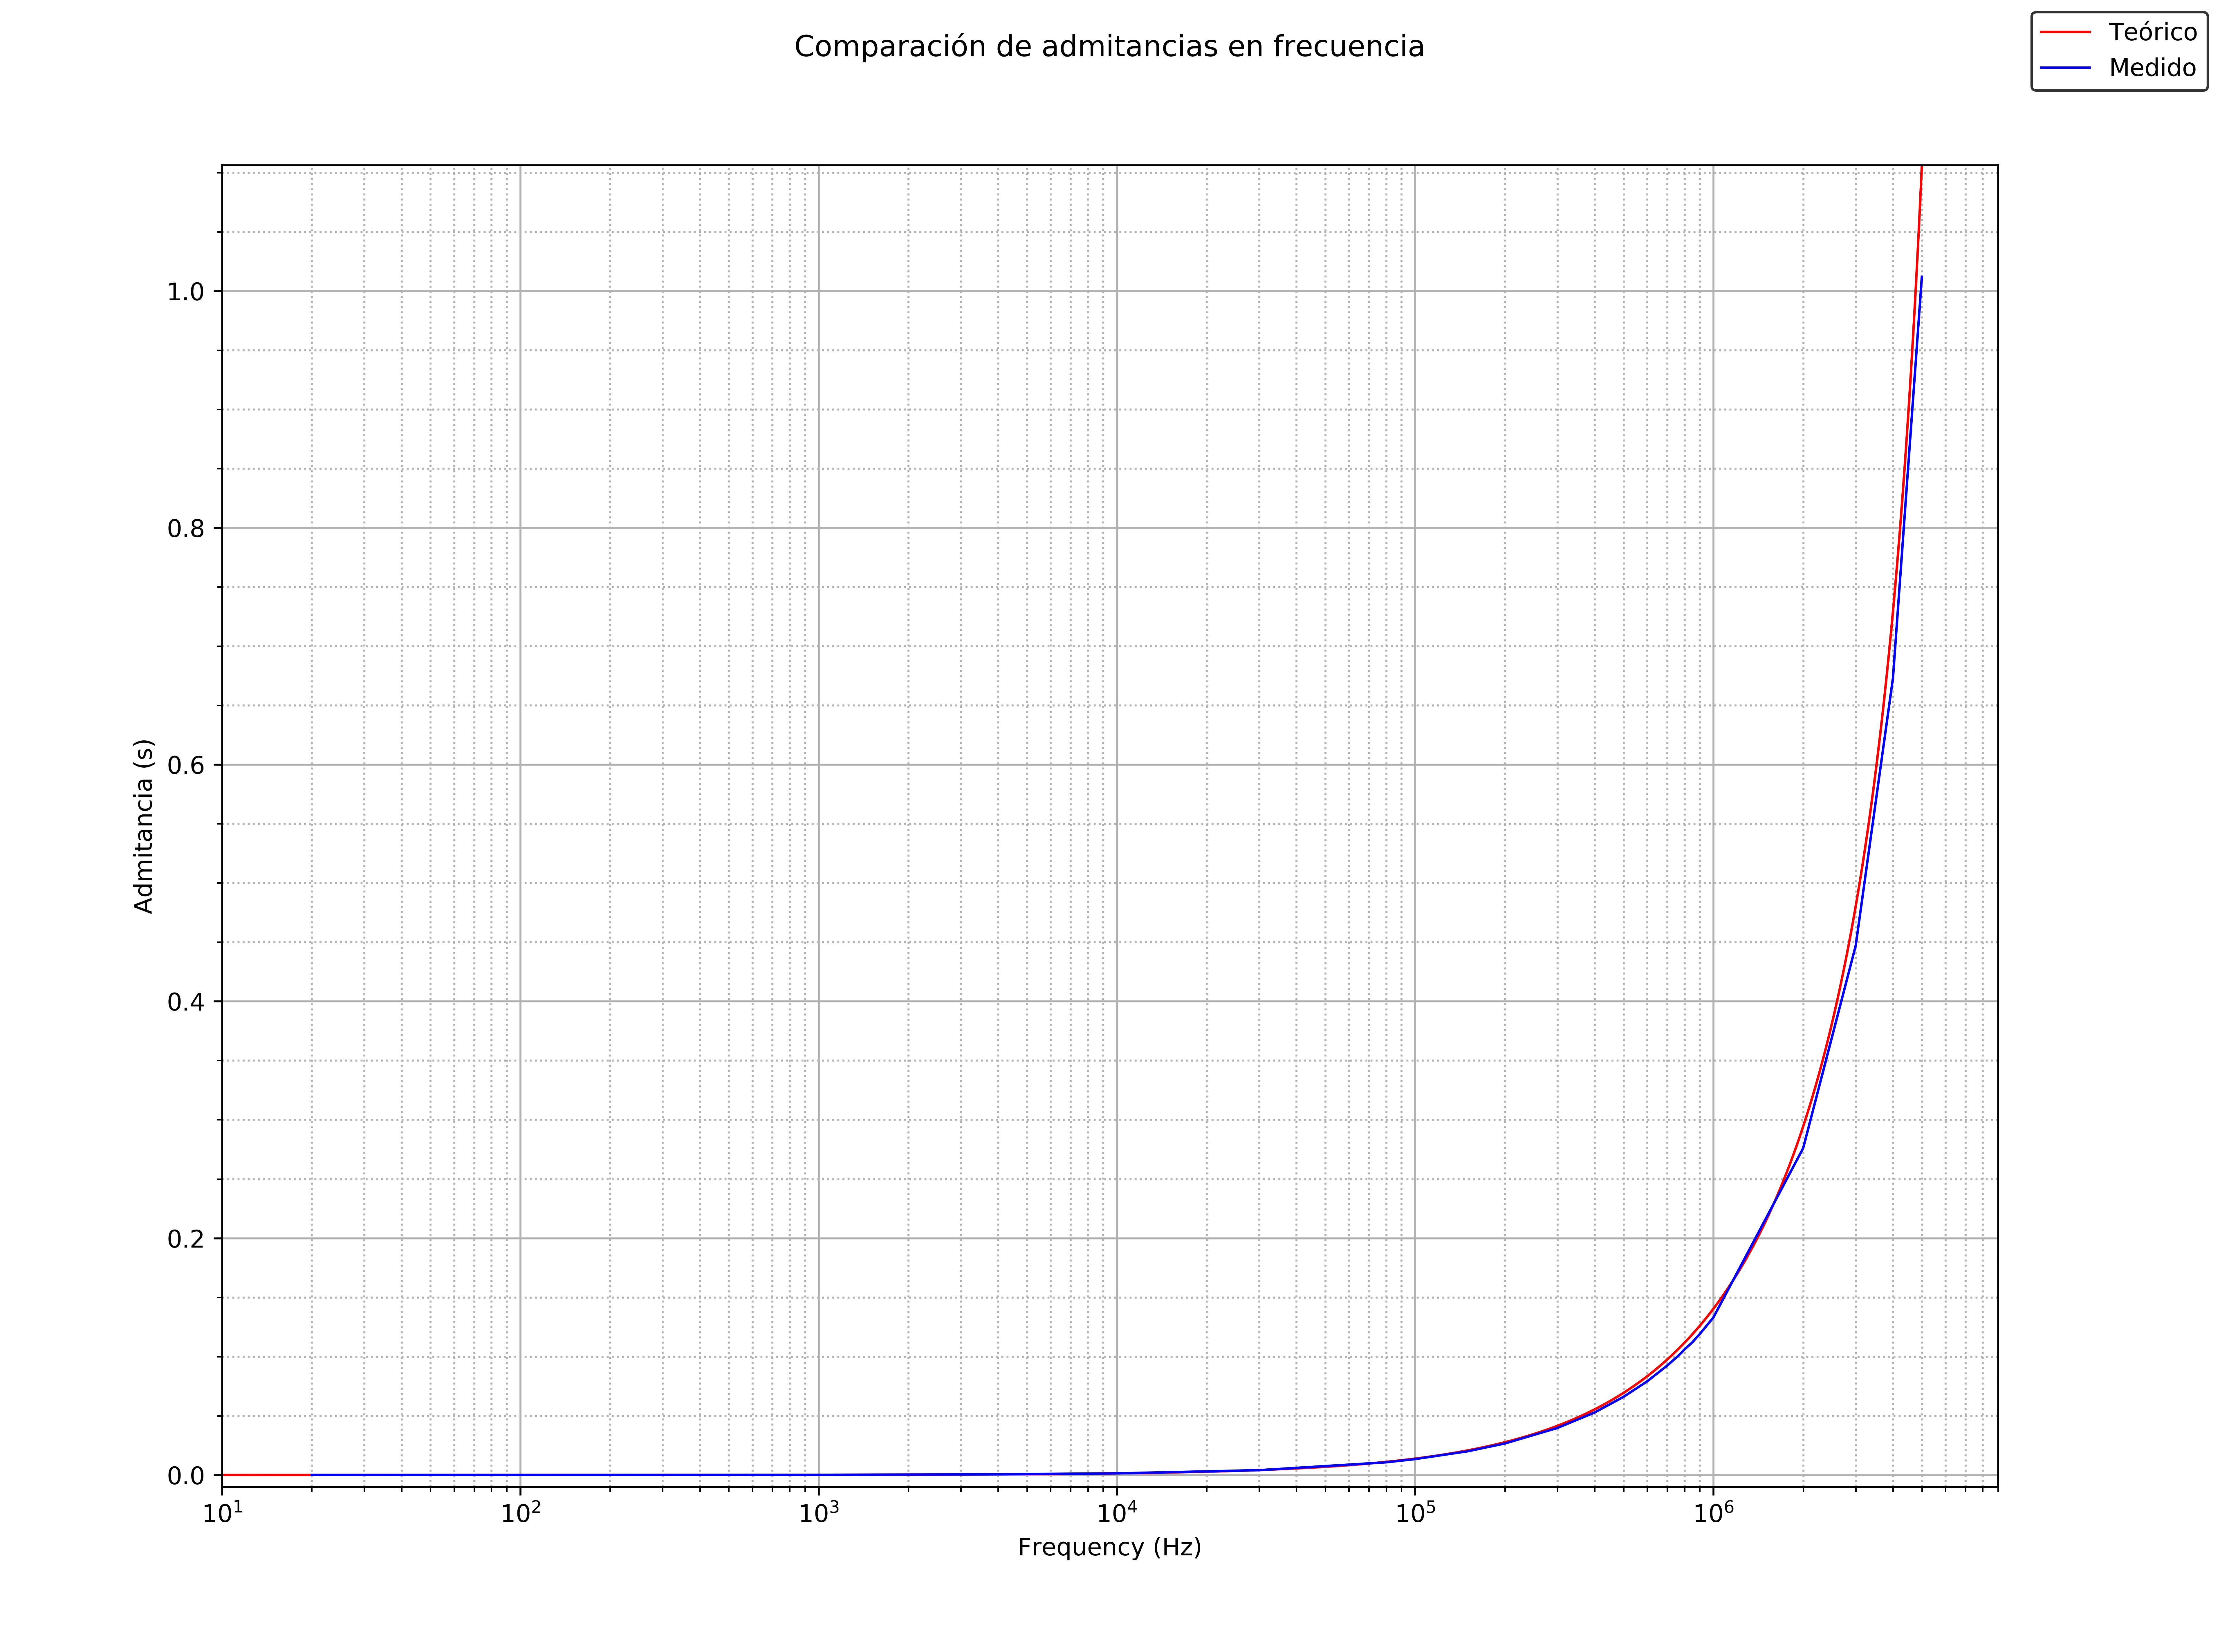
\includegraphics{Recursos/comp_admitancia_cap.png} &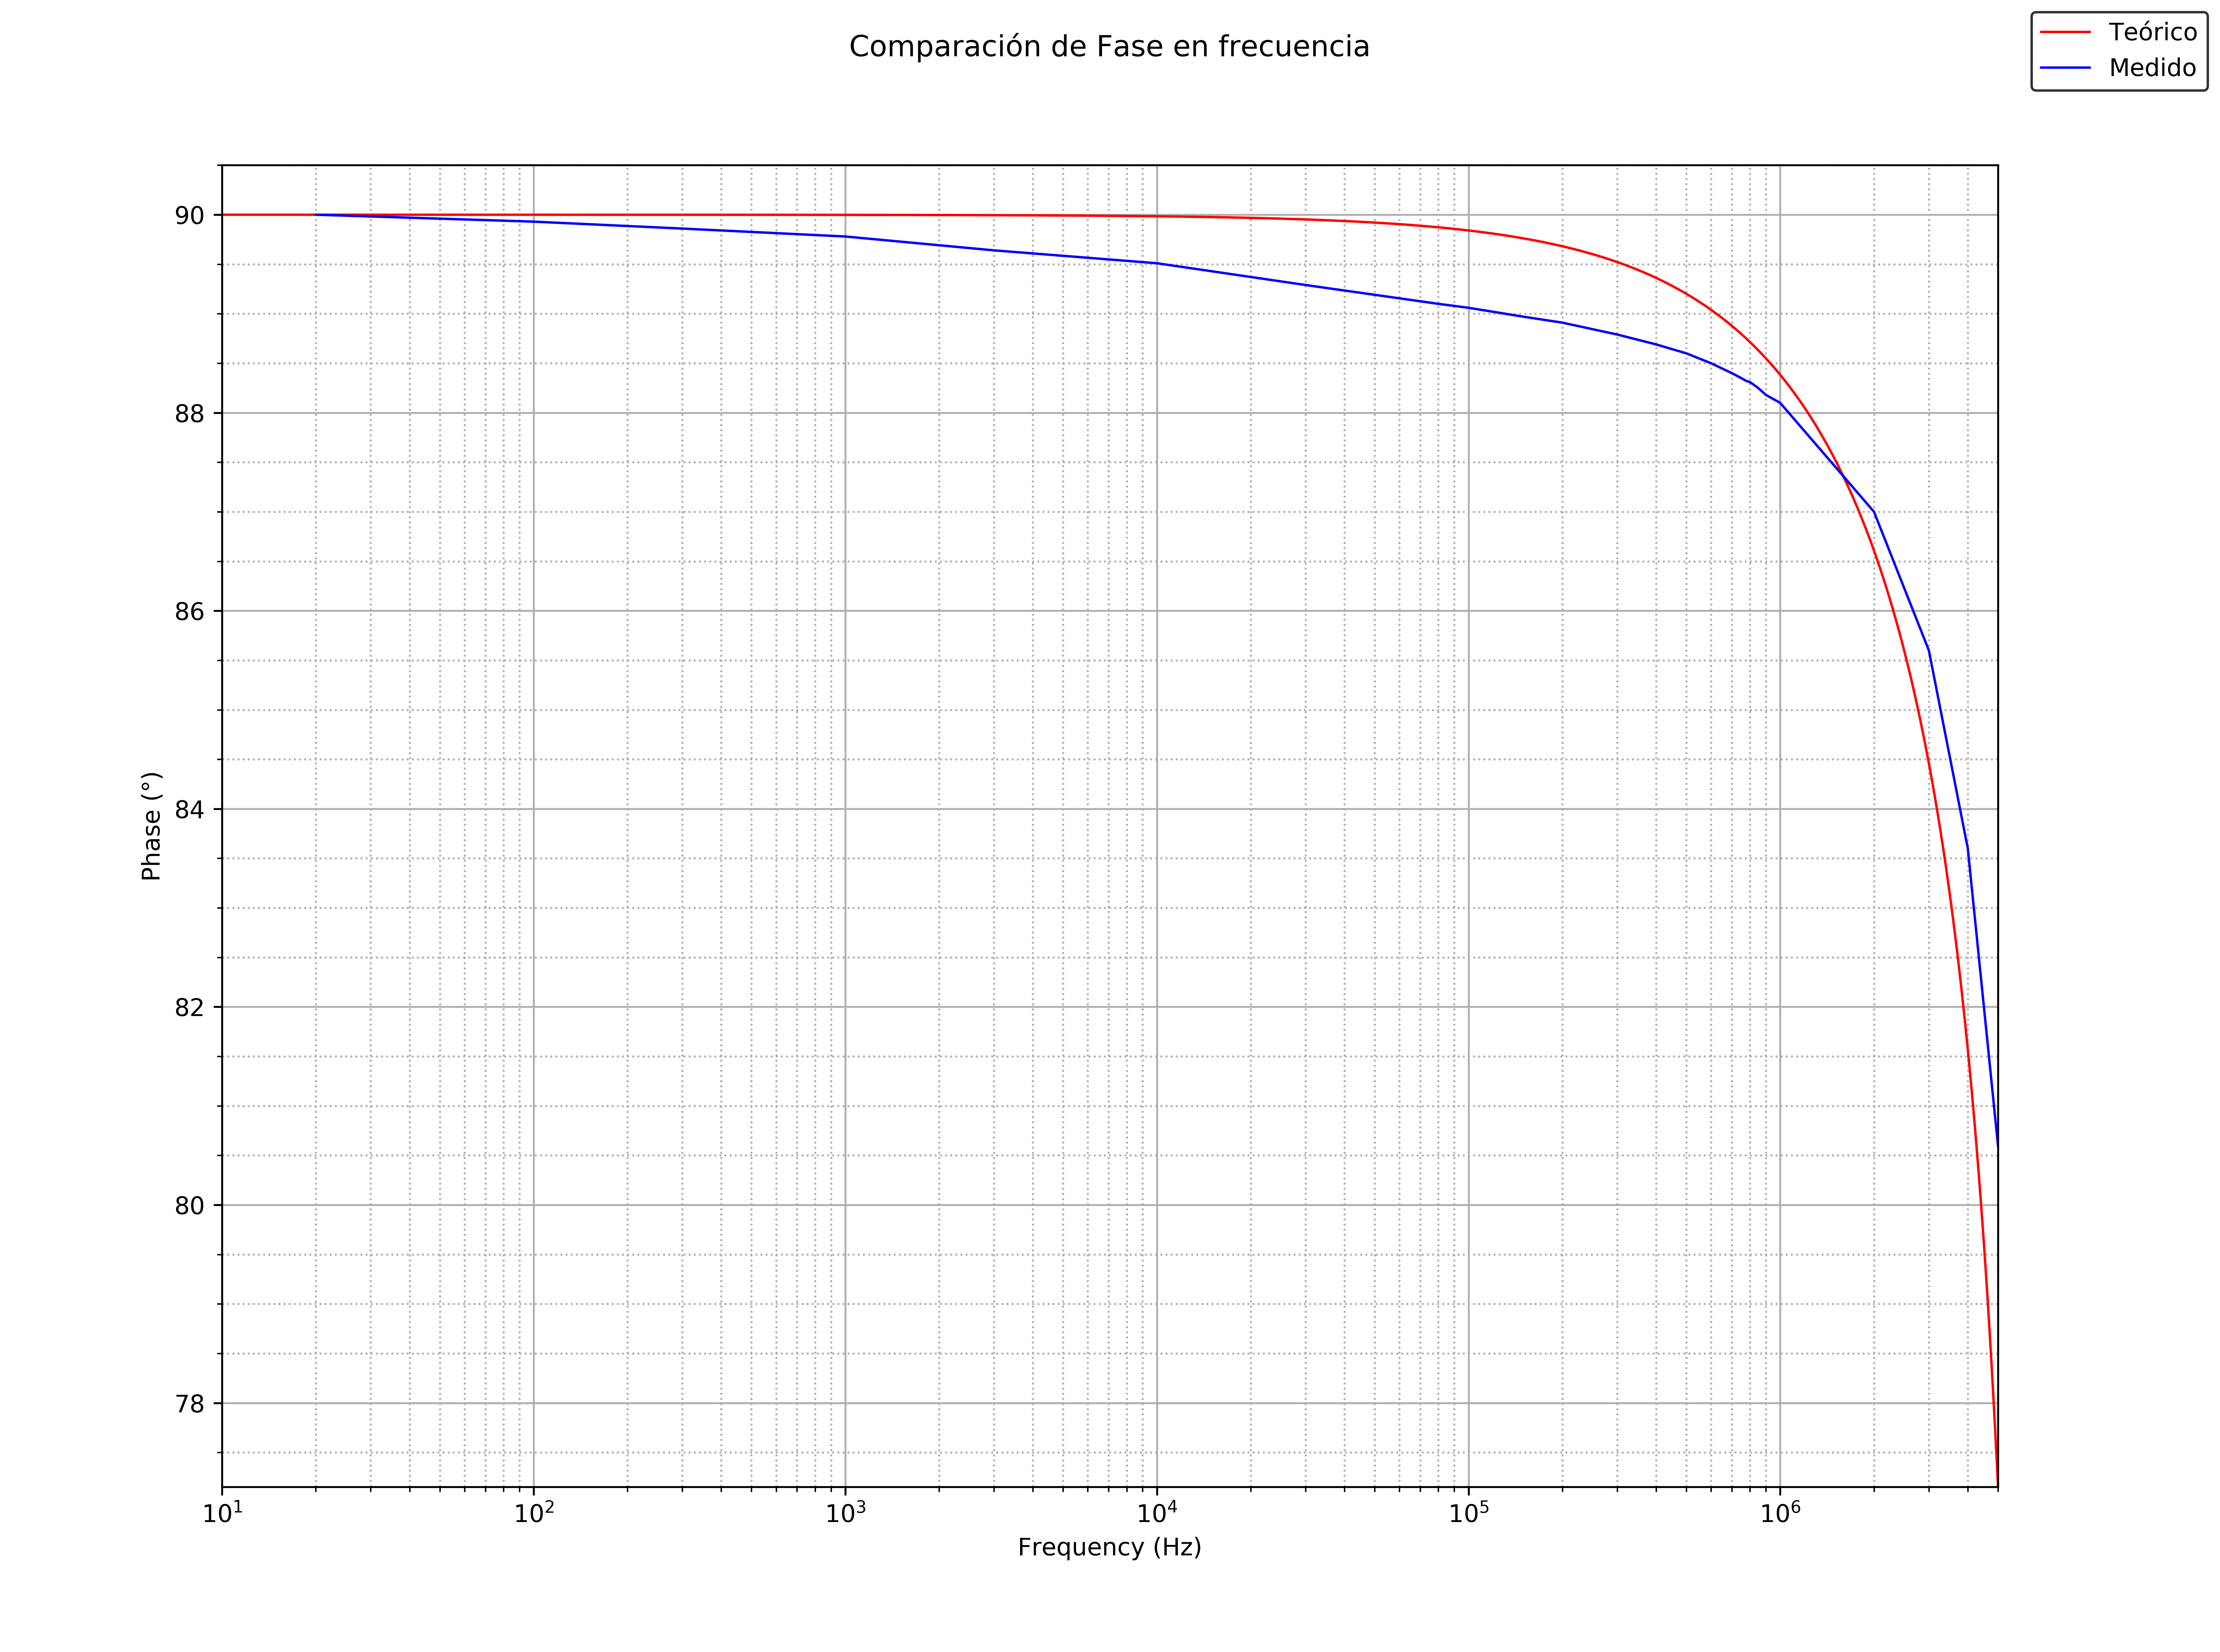
\includegraphics{Recursos/comp_fase_cap.png}
        \end{tabular}
        
    }
    \caption{Comparaci\'on entre mediciones y modelo de admitancia y fase en funci\'on de la frecuencia. }
        \label{fig:Comp_CAP}    
\end{figure}
Se observa un ajuste correcto en la comparaci\'on del modelo con las mediciones en el caso de la admitancia, lo que se corresponde con lo esperado ya que se dise\~na el circuito con ese fin. 

Si bien el comportamiento de la fase no coincide exactamente con el modelo, se puede observar que la forma es correcta. Se asume que estas diferencias son causadas por fen\'omenos no analizados en el capacitor como por ejemplo la variaci\'on de los valores de ESR y ESL con la frecuencia.

\subsection{Medici\'on del inductor}
Para la medici\'on se utiliza un inductor de $500\mu H$ con n\'ucleo de ferrite y se configura el analizador de impedancias en modelo serie para medir fase e impedancia. 
\subsubsection{Resultados}
Se muestran en la Tabla \ref{tab:Med_IND}  los resultados obtenidos de las mediciones y en la Figura \ref{fig:Med_IND} los respectivos  gr\'aficos realizados a partir de estas.
\begin{table}[H]
    \centering
    \resizebox{0.5\textwidth}{!}{%
        \begin{tabular}{ccccc}
            \hline
            \begin{tabular}[c]{@{}c@{}}Frecuencia\\   (Hz)
            \end{tabular} & Inductancia (Hy) & \begin{tabular}[c]{@{}c@{}}Factor de\\   calidad (Q)\end{tabular} & \multicolumn{1}{l}{Impedancia ($\Omega$)} & Fase ($^\circ$) \\ \hline
            10 & 5.00E-04 & 0 & 0.1 & 18.2 \\
            20 & 4.90E-04 & 1 & 1.13E-01 & 33 \\
            100 & 4.96E-04 & 3 & 0.328 & 71.6 \\
            300 & 4.92E-04 & 8 & 9.35E-01 & 82.6 \\
            1000 & 4.94E-04 & 16 & 3.11 & 86.4 \\
            3000 & 4.89E-04 & 23.5 & 9.23E+00 & 87.54 \\
            10000 & 4.89E-04 & 25 & 30.77 & 87.67 \\
            30000 & 4.77E-04 & 22.5 & 9.02E+01 & 87.43 \\
            80000 & 4.64E-04 & 17 & 2.34E+02 & 86.6 \\
            100000 & 4.66E-04 & 14.7 & 293 & 86.09 \\
            150000 & 4.66E-04 & 11.3 & 4.41E+02 & 84.93 \\
            200000 & 4.73E-04 & 8.9 & 5.98E+02 & 83.57 \\
            300000 & 5.00E-04 & 5.9 & 9.56E+02 & 80.47 \\
            400000 & 5.47E-04 & 4.1 & 1.41E+03 & 76.42 \\
            500000 & 6.20E-04 & 2.9 & 2.06E+03 & 70.7 \\
            600000 & 7.15E-04 & 1.8 & 3.07E+03 & 61.5 \\
            700000 & 7.52E-04 & 1 & 4.73E+03 & 44.4 \\
            750000 & 6.18E-04 & 0.6 & 5.80E+03 & 30.24 \\
            780000 & 4.32E-04 & 0.4 & 6.37E+03 & 19.4 \\
            800000 & 2.56E-04 & 0.2 & 6.66E+03 & 11.11 \\
            825000 & 2.30E-05 & 0 & 6.84E+03 & 1.04 \\
            850000 & -2.05E-04 & 0.2 & 6.78E+03 & -9.29 \\
            875000 & -3.80E-04 & 0.3 & 6.54E+03 & -18.86 \\
            900000 & -5.03E-04 & 0.5 & 6.16E+03 & -27.5 \\
            950000 & -5.82E-04 & 0.9 & 5.31E+03 & -40.89 \\
            1000000 & -5.53E-04 & 1.2 & 4.48E+03 & -50.73 \\
            1250000 & -2.90E-04 & 2.8 & 2.47E+03 & -70.5 \\
            1500000 & -1.70E-04 & 4.4 & 1.71E+03 & -77.11 \\
            1650000 & -1.38E-04 & 5.3 & 1.46E+03 & -79.25 \\
            1750000 & -1.19E-04 & 5.8 & 1.33E+03 & -80.31 \\
            2000000 & -8.59E-05 & 7.3 & 1.08E+03 & -82.24 \\
            3000000 & -3.43E-05 & 12.8 & 6.48E+02 & -85.51 \\
            4000000 & -1.86E-05 & 17.5 & 4.66E+02 & -86.7 \\
            5000000 & -1.16E-05 & 21.2 & 3.65E+02 & -87.27 \\
            10000000 & -2.70E-06 & 24.6 & 170.4 & -87.64 \\ \hline
        \end{tabular}%
    }
    \caption{Mediciones del inductor}
    \label{tab:Med_IND}
\end{table}
\begin{figure}[H]
    \centering
    \resizebox{\textwidth}{!}{
        \begin{tabular}{c c}
            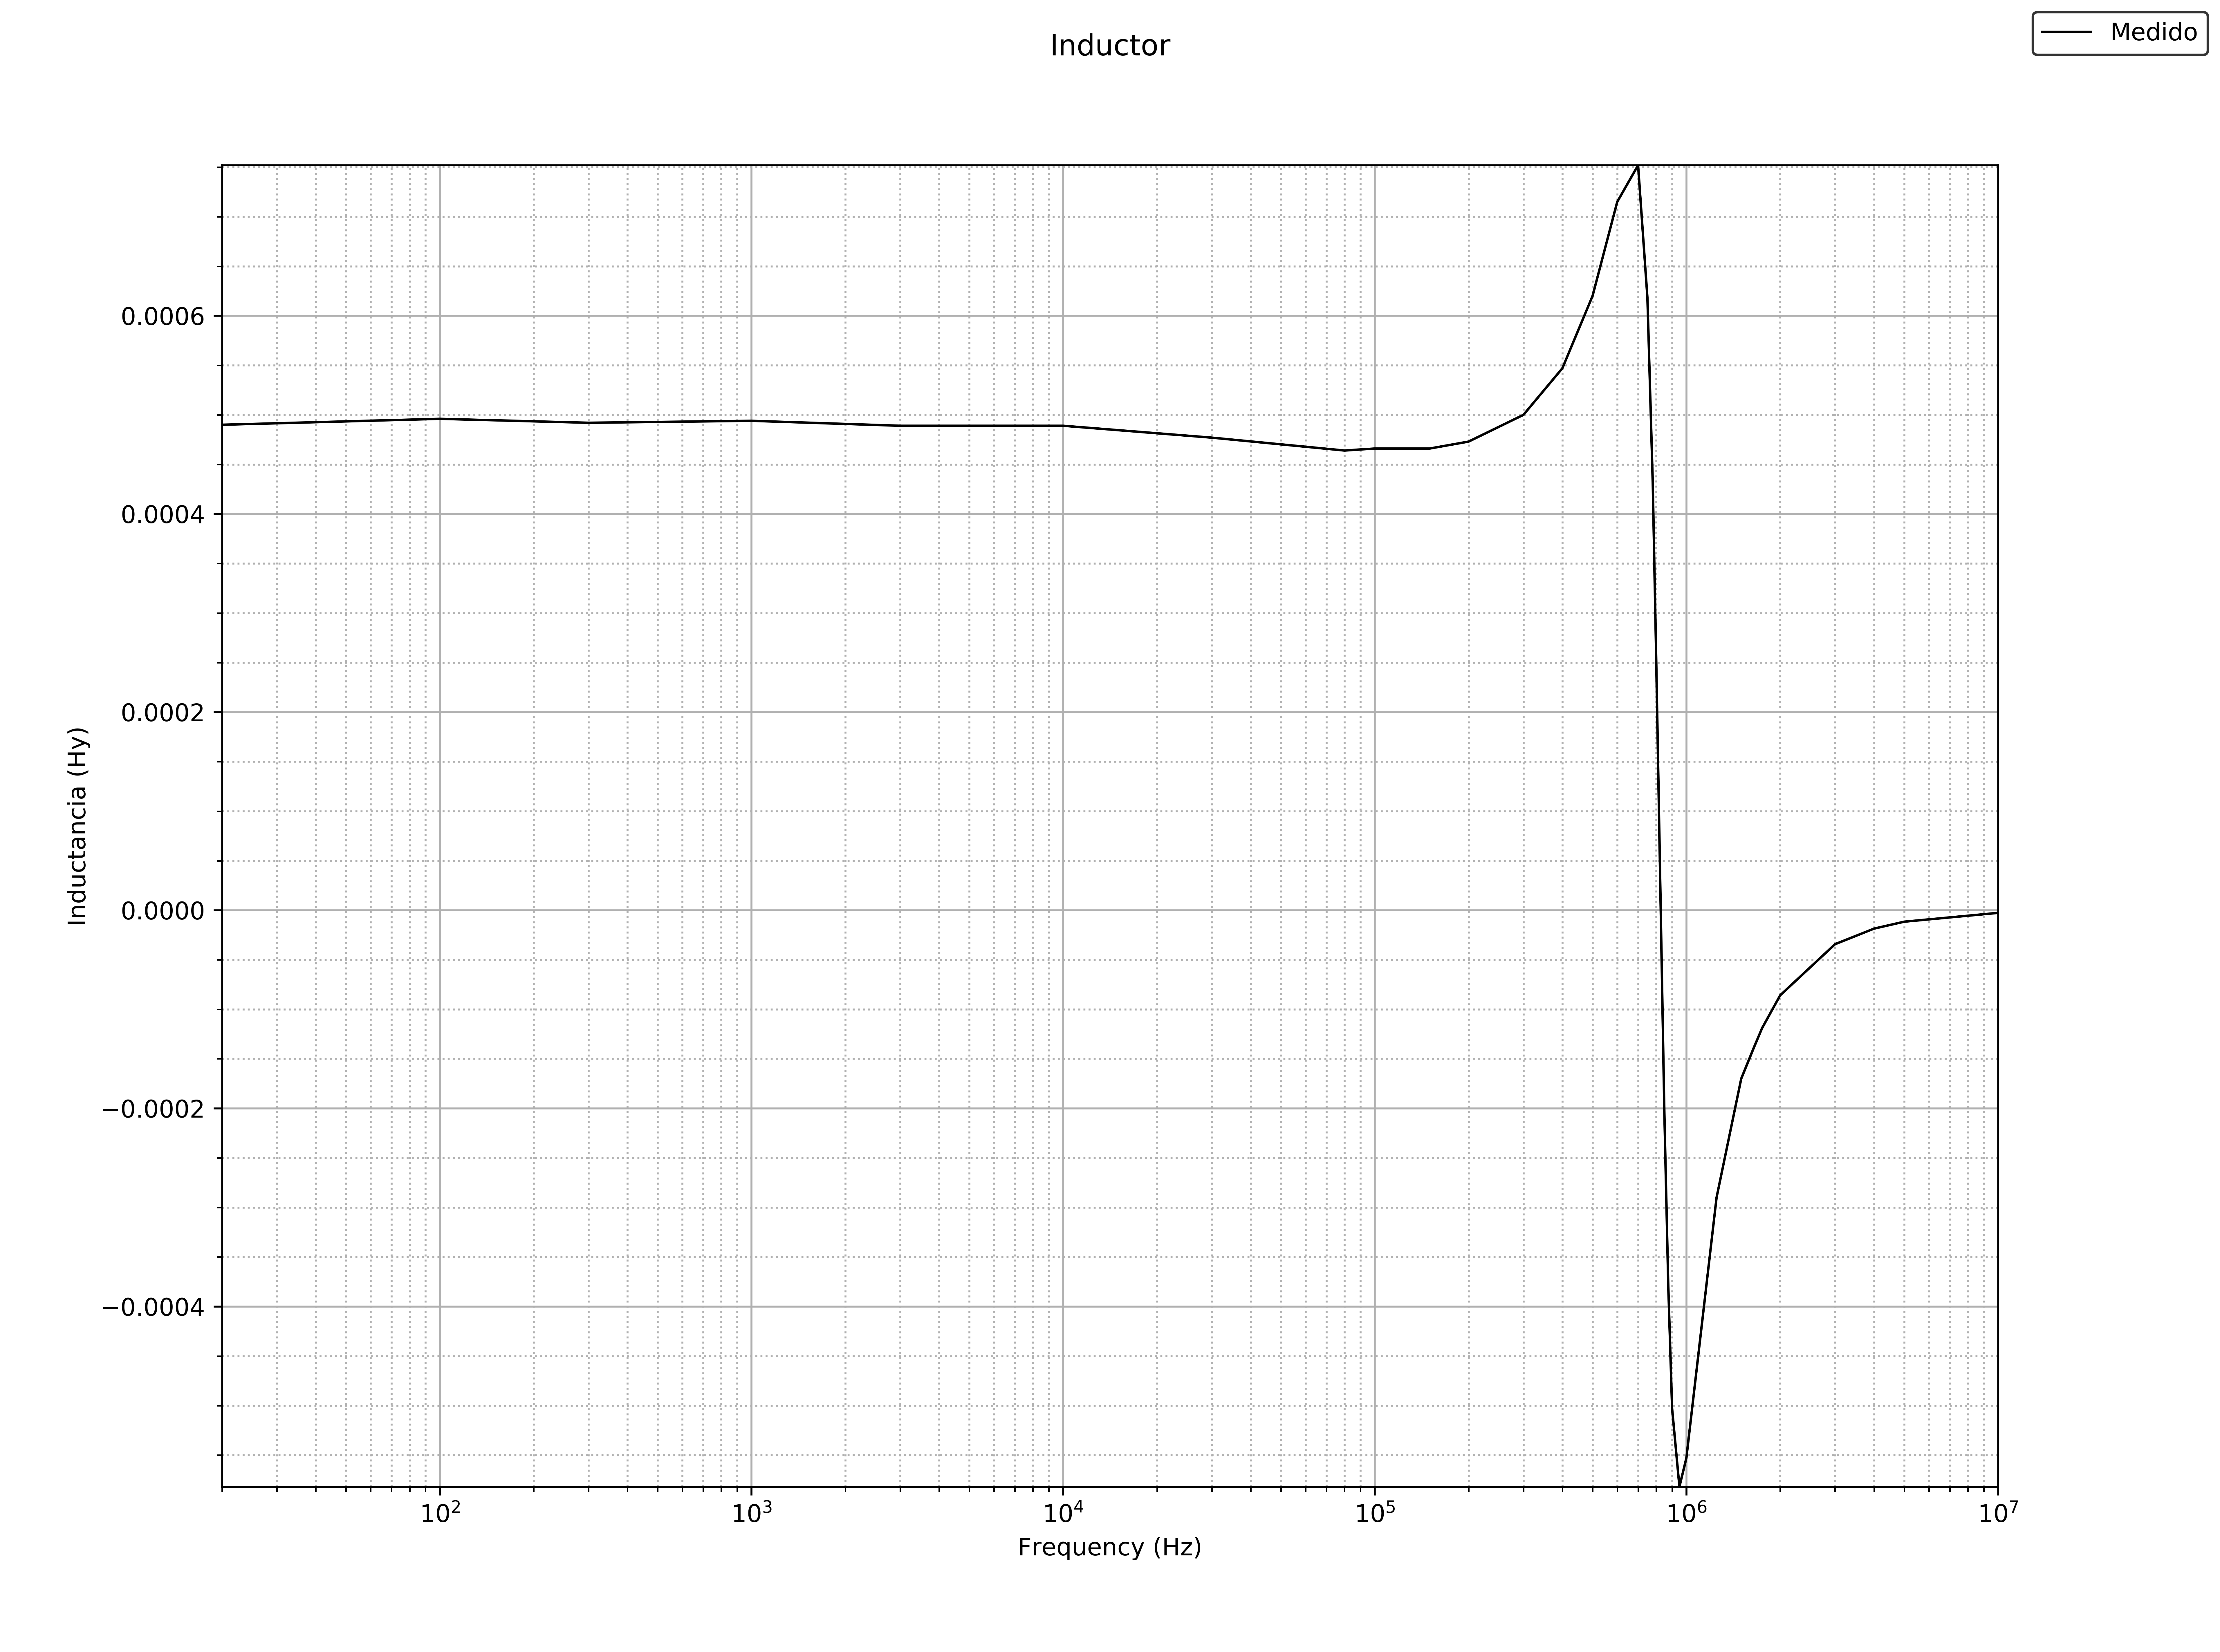
\includegraphics{Recursos/inductancia_medida_ind.png}&
            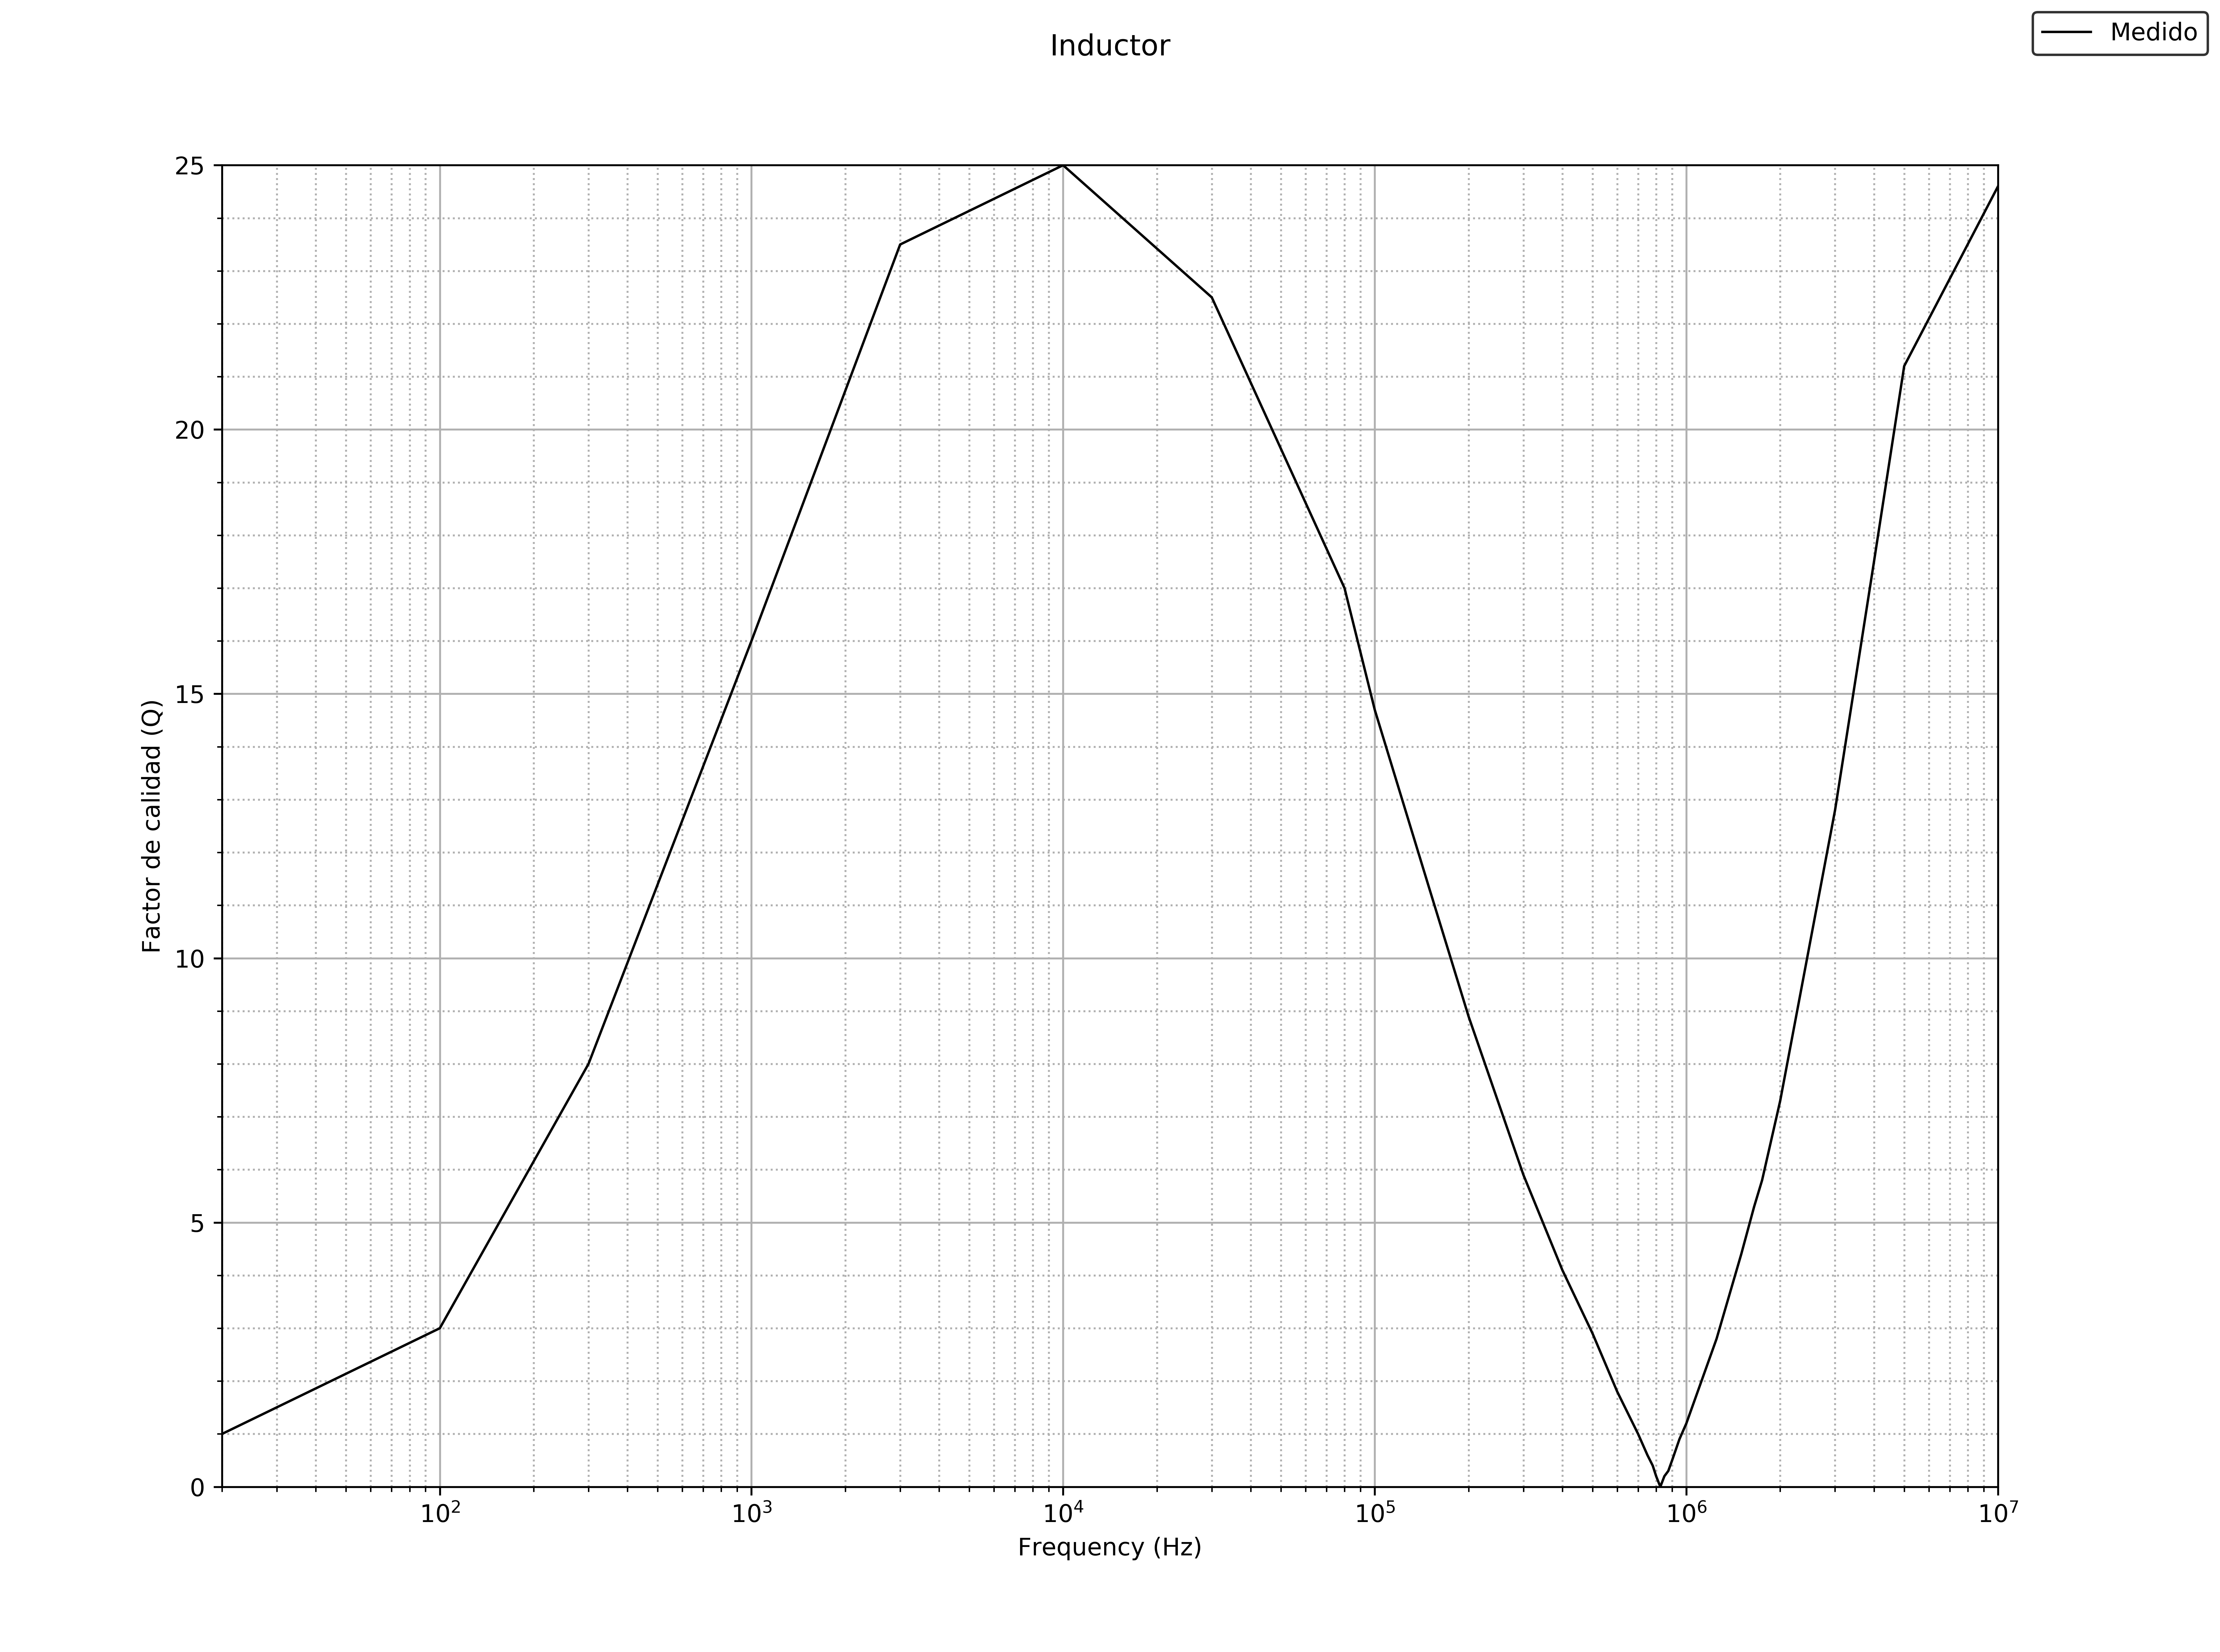
\includegraphics{Recursos/calidad_medida_ind.png} \\
            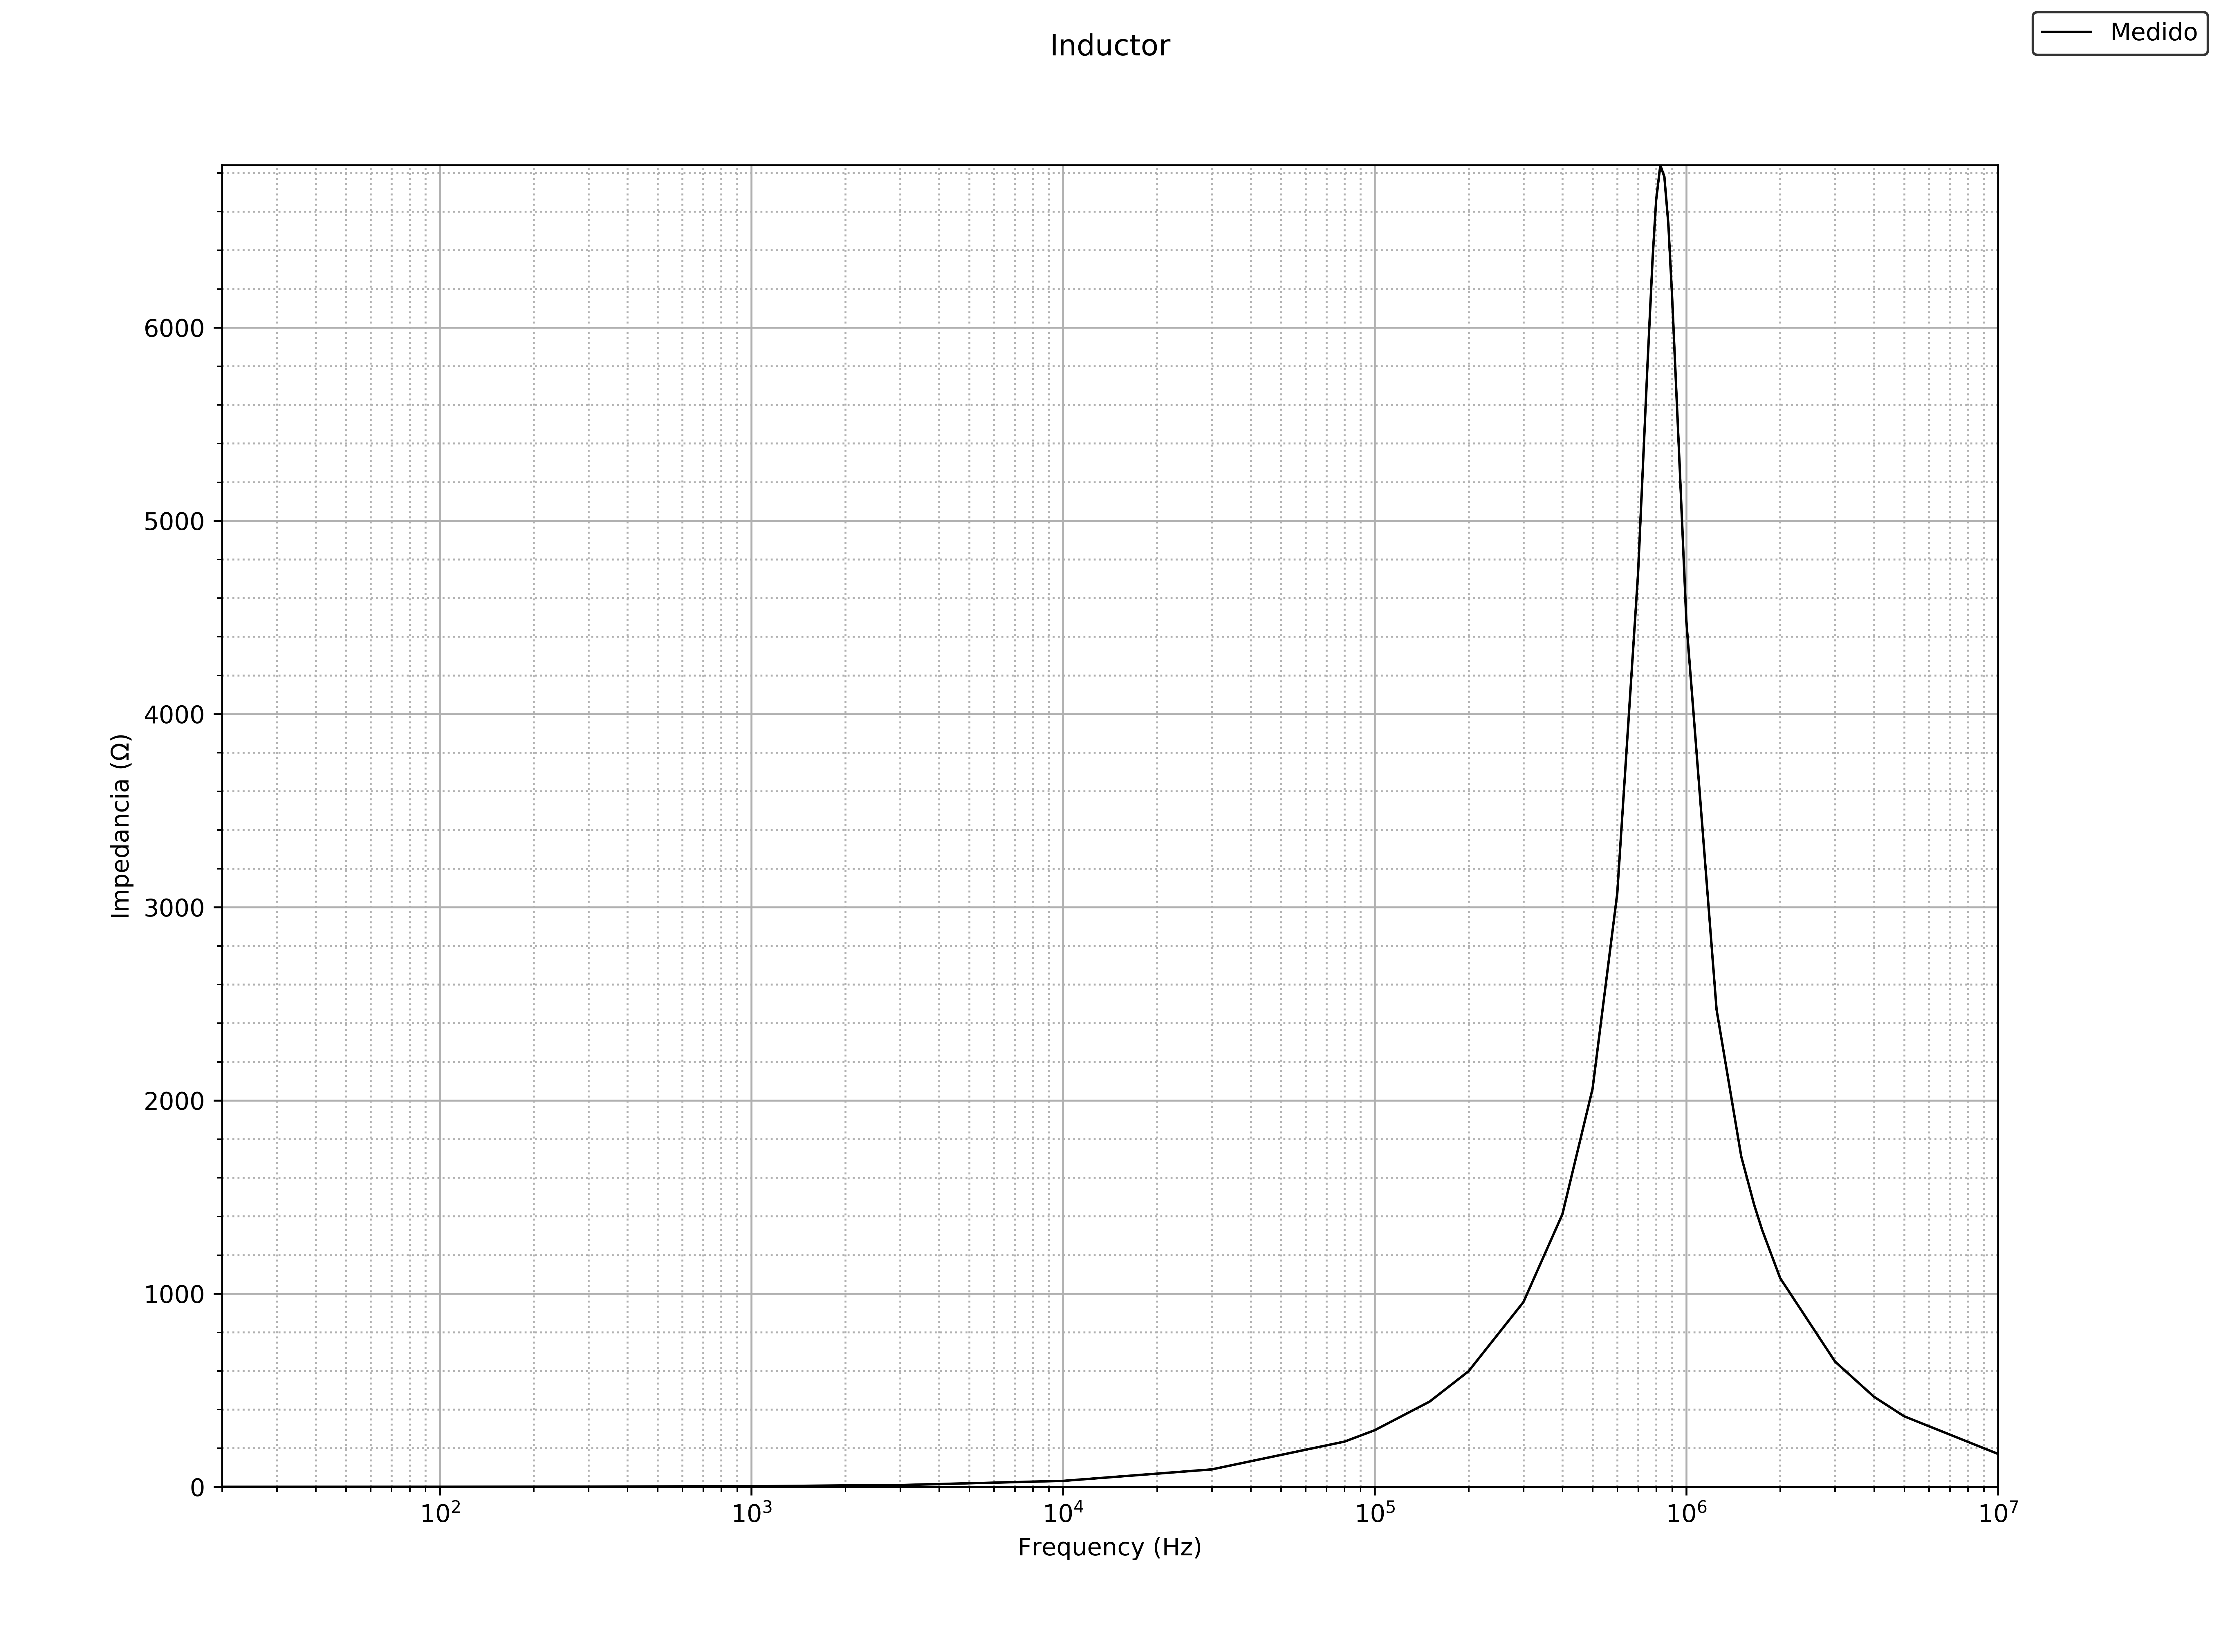
\includegraphics{Recursos/impedancia_medida_ind.png} &
            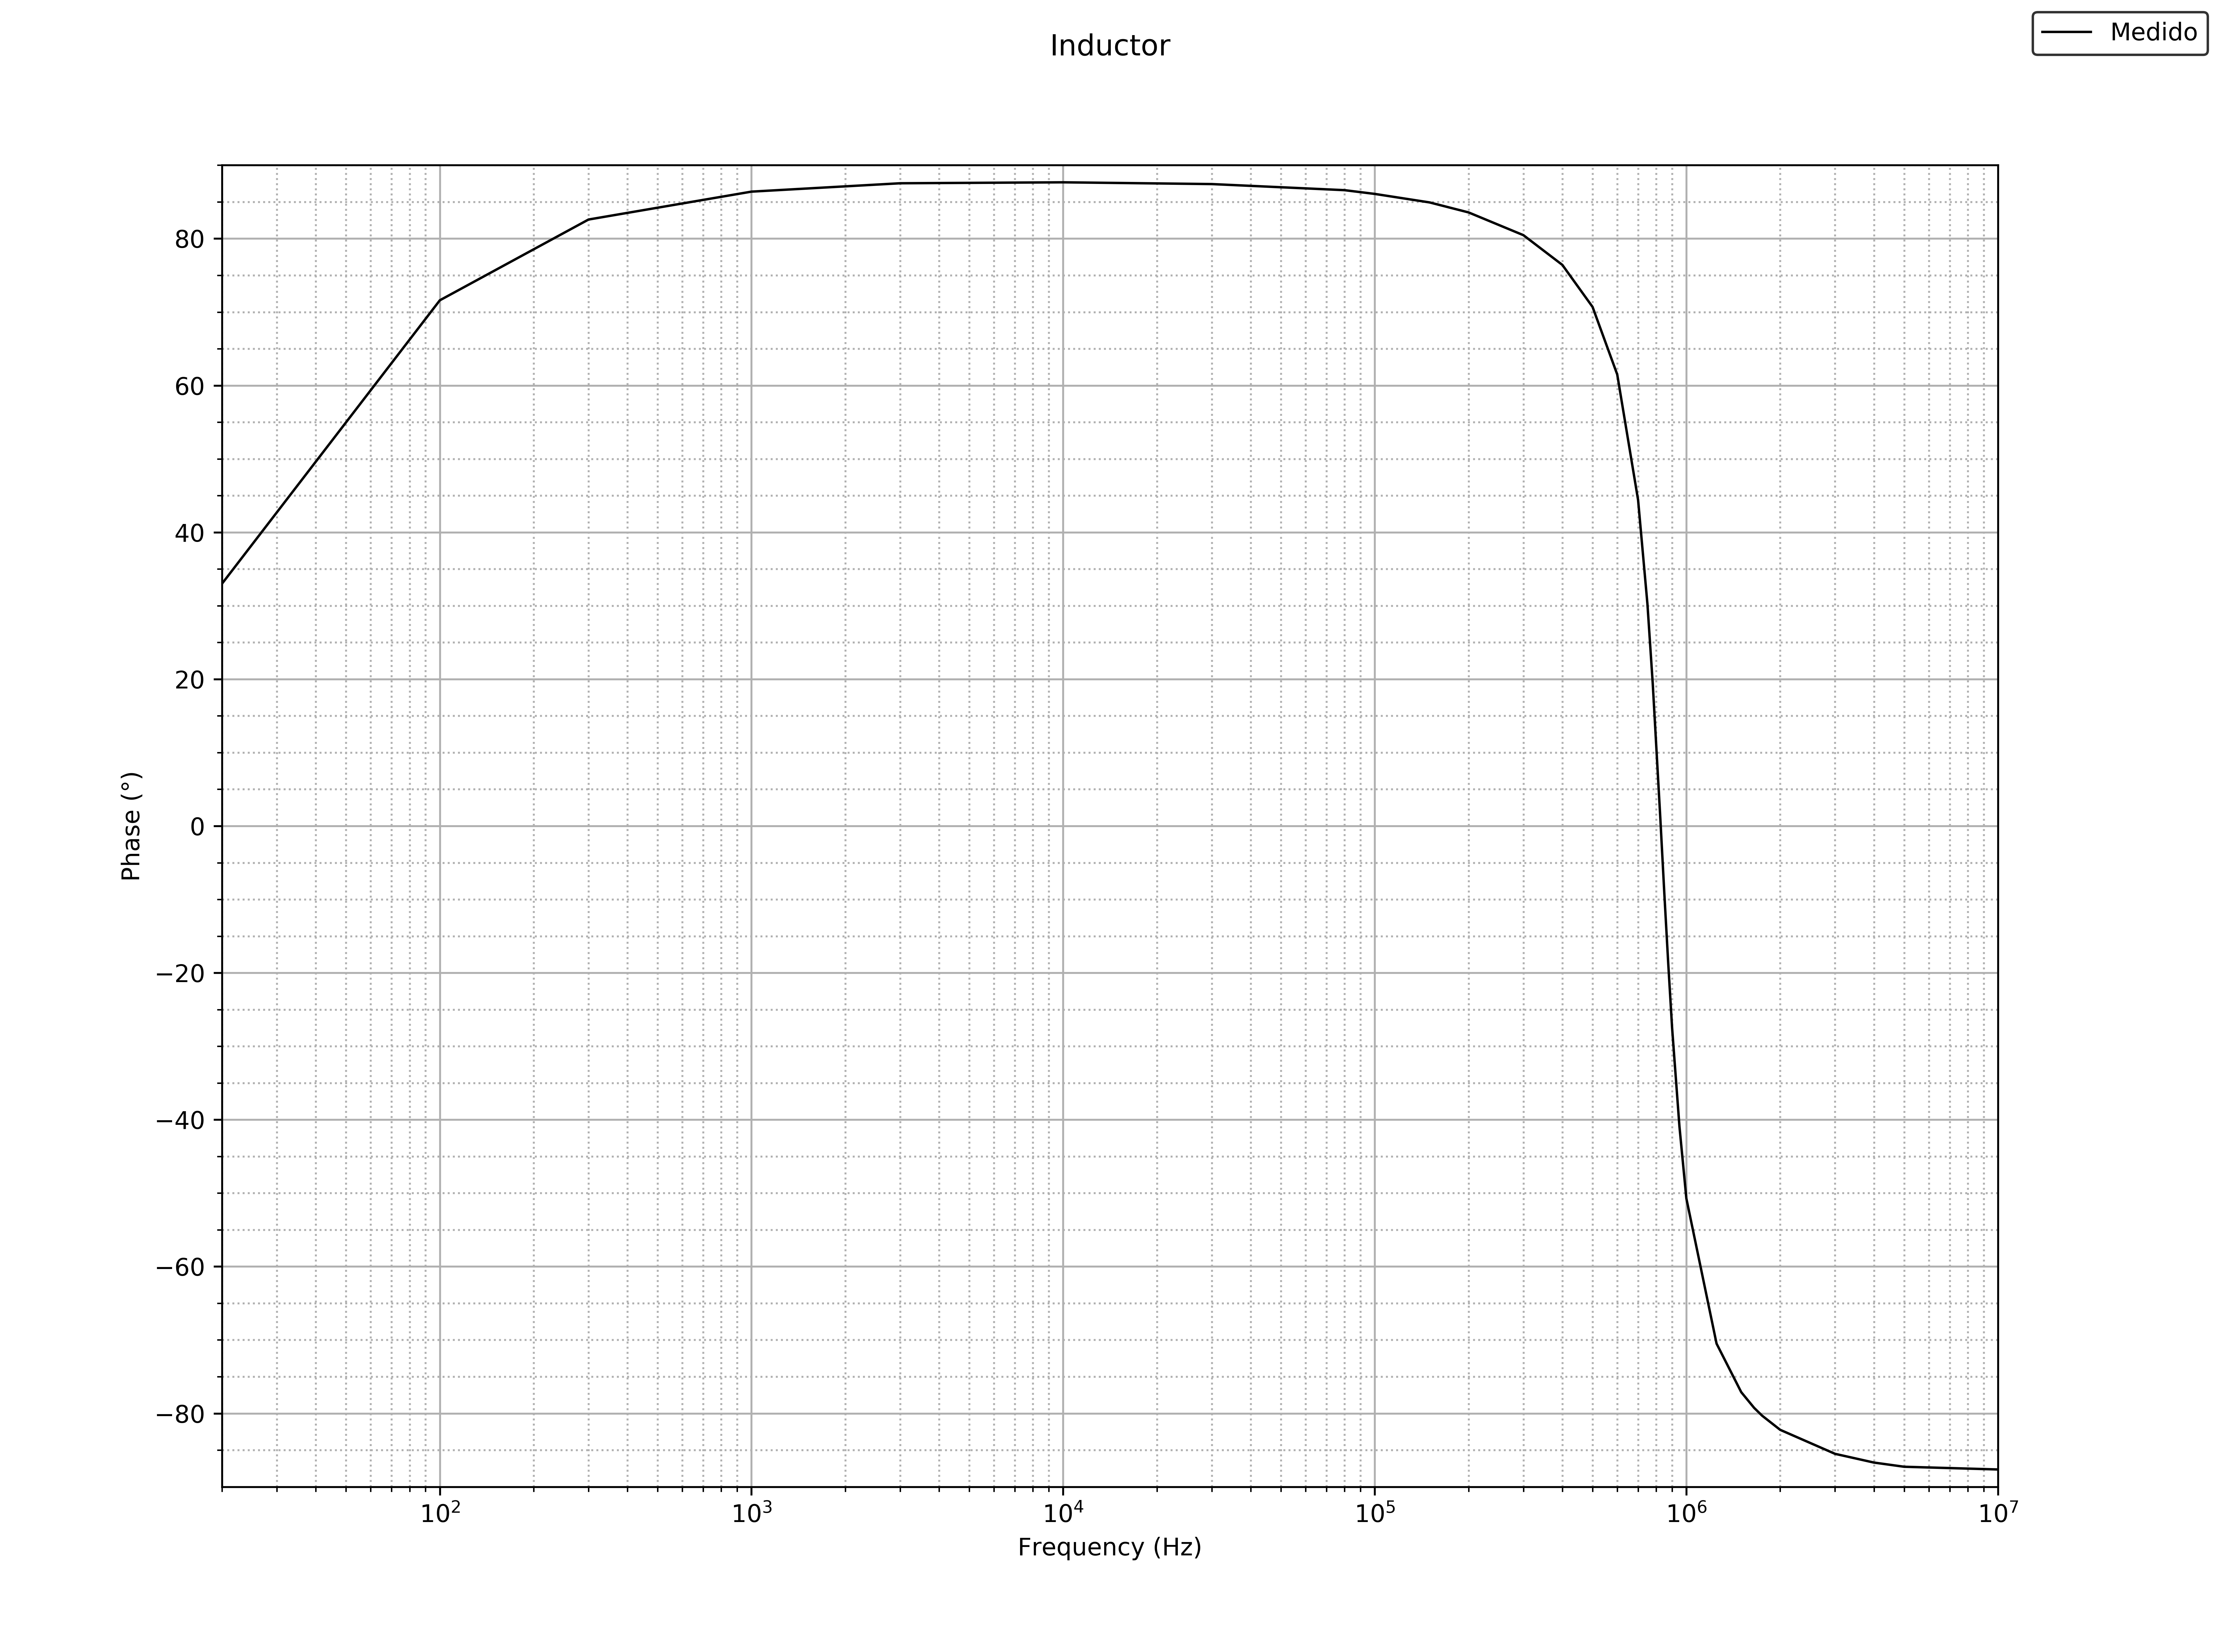
\includegraphics{Recursos/fase_medida_ind.png}

        \end{tabular}
    }
    \caption{Gr\'aficos realizados a partir de las mediciones}
    \label{fig:Med_IND}
        
\end{figure}    

\subsubsection{Modelizaci\'on del comportamiento observado}
Se propone el circuito de la Figura \ref{fig:modelo_IND} con el fin de encontrar un modelo que se ajuste al comportamiento real del inductor tanto en impedancia como en fase.
\begin{figure}[H]
    \centering
    \resizebox{0.5\textwidth}{!}{
        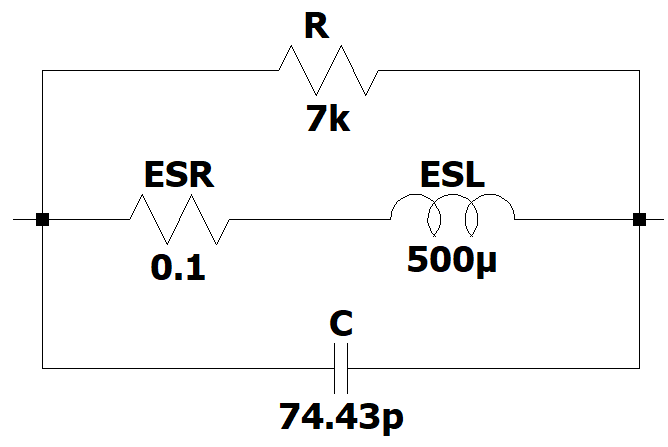
\includegraphics{Recursos/Modelo_ind.png}
    }
    \caption{Modelo de comportamiento del inductor}
    \label{fig:modelo_IND}
\end{figure}
Asumiendo que el valor de la inductancia es de $500\mu Hy$, lo cual es correcto si se tiene en cuanta que para frecuencias medias ese es el valor que se obtuvo en las mediciones, se puede encontrar un valor para $C$ de igual forma que para el modelo del capacitor y tomando el valor para la frecuencia de corte $f_0 = 825KHz$ que nuevamente es el valor para el cual la inductancia medida con el analizador de impedancias pasa de positiva a negativa.

Para los valores de $ESR$ y $R$ se eligen valores de manera que para frecuencias bajas la resistencia equivalente del modelo coincida con la impedancia medida, y se fija el valor $R = 7K\Omega$ para lograr un mejor ajuste a la curva medida, limitando la m\'axima impedancia del modelo.

Se muestran en la Figura \ref{fig:Comp_IND}, los resultados obtenidos a partir del modelo elegido.
\begin{figure}[H]
    \centering
    \resizebox{\textwidth}{!}{
        \begin{tabular}{c c}
            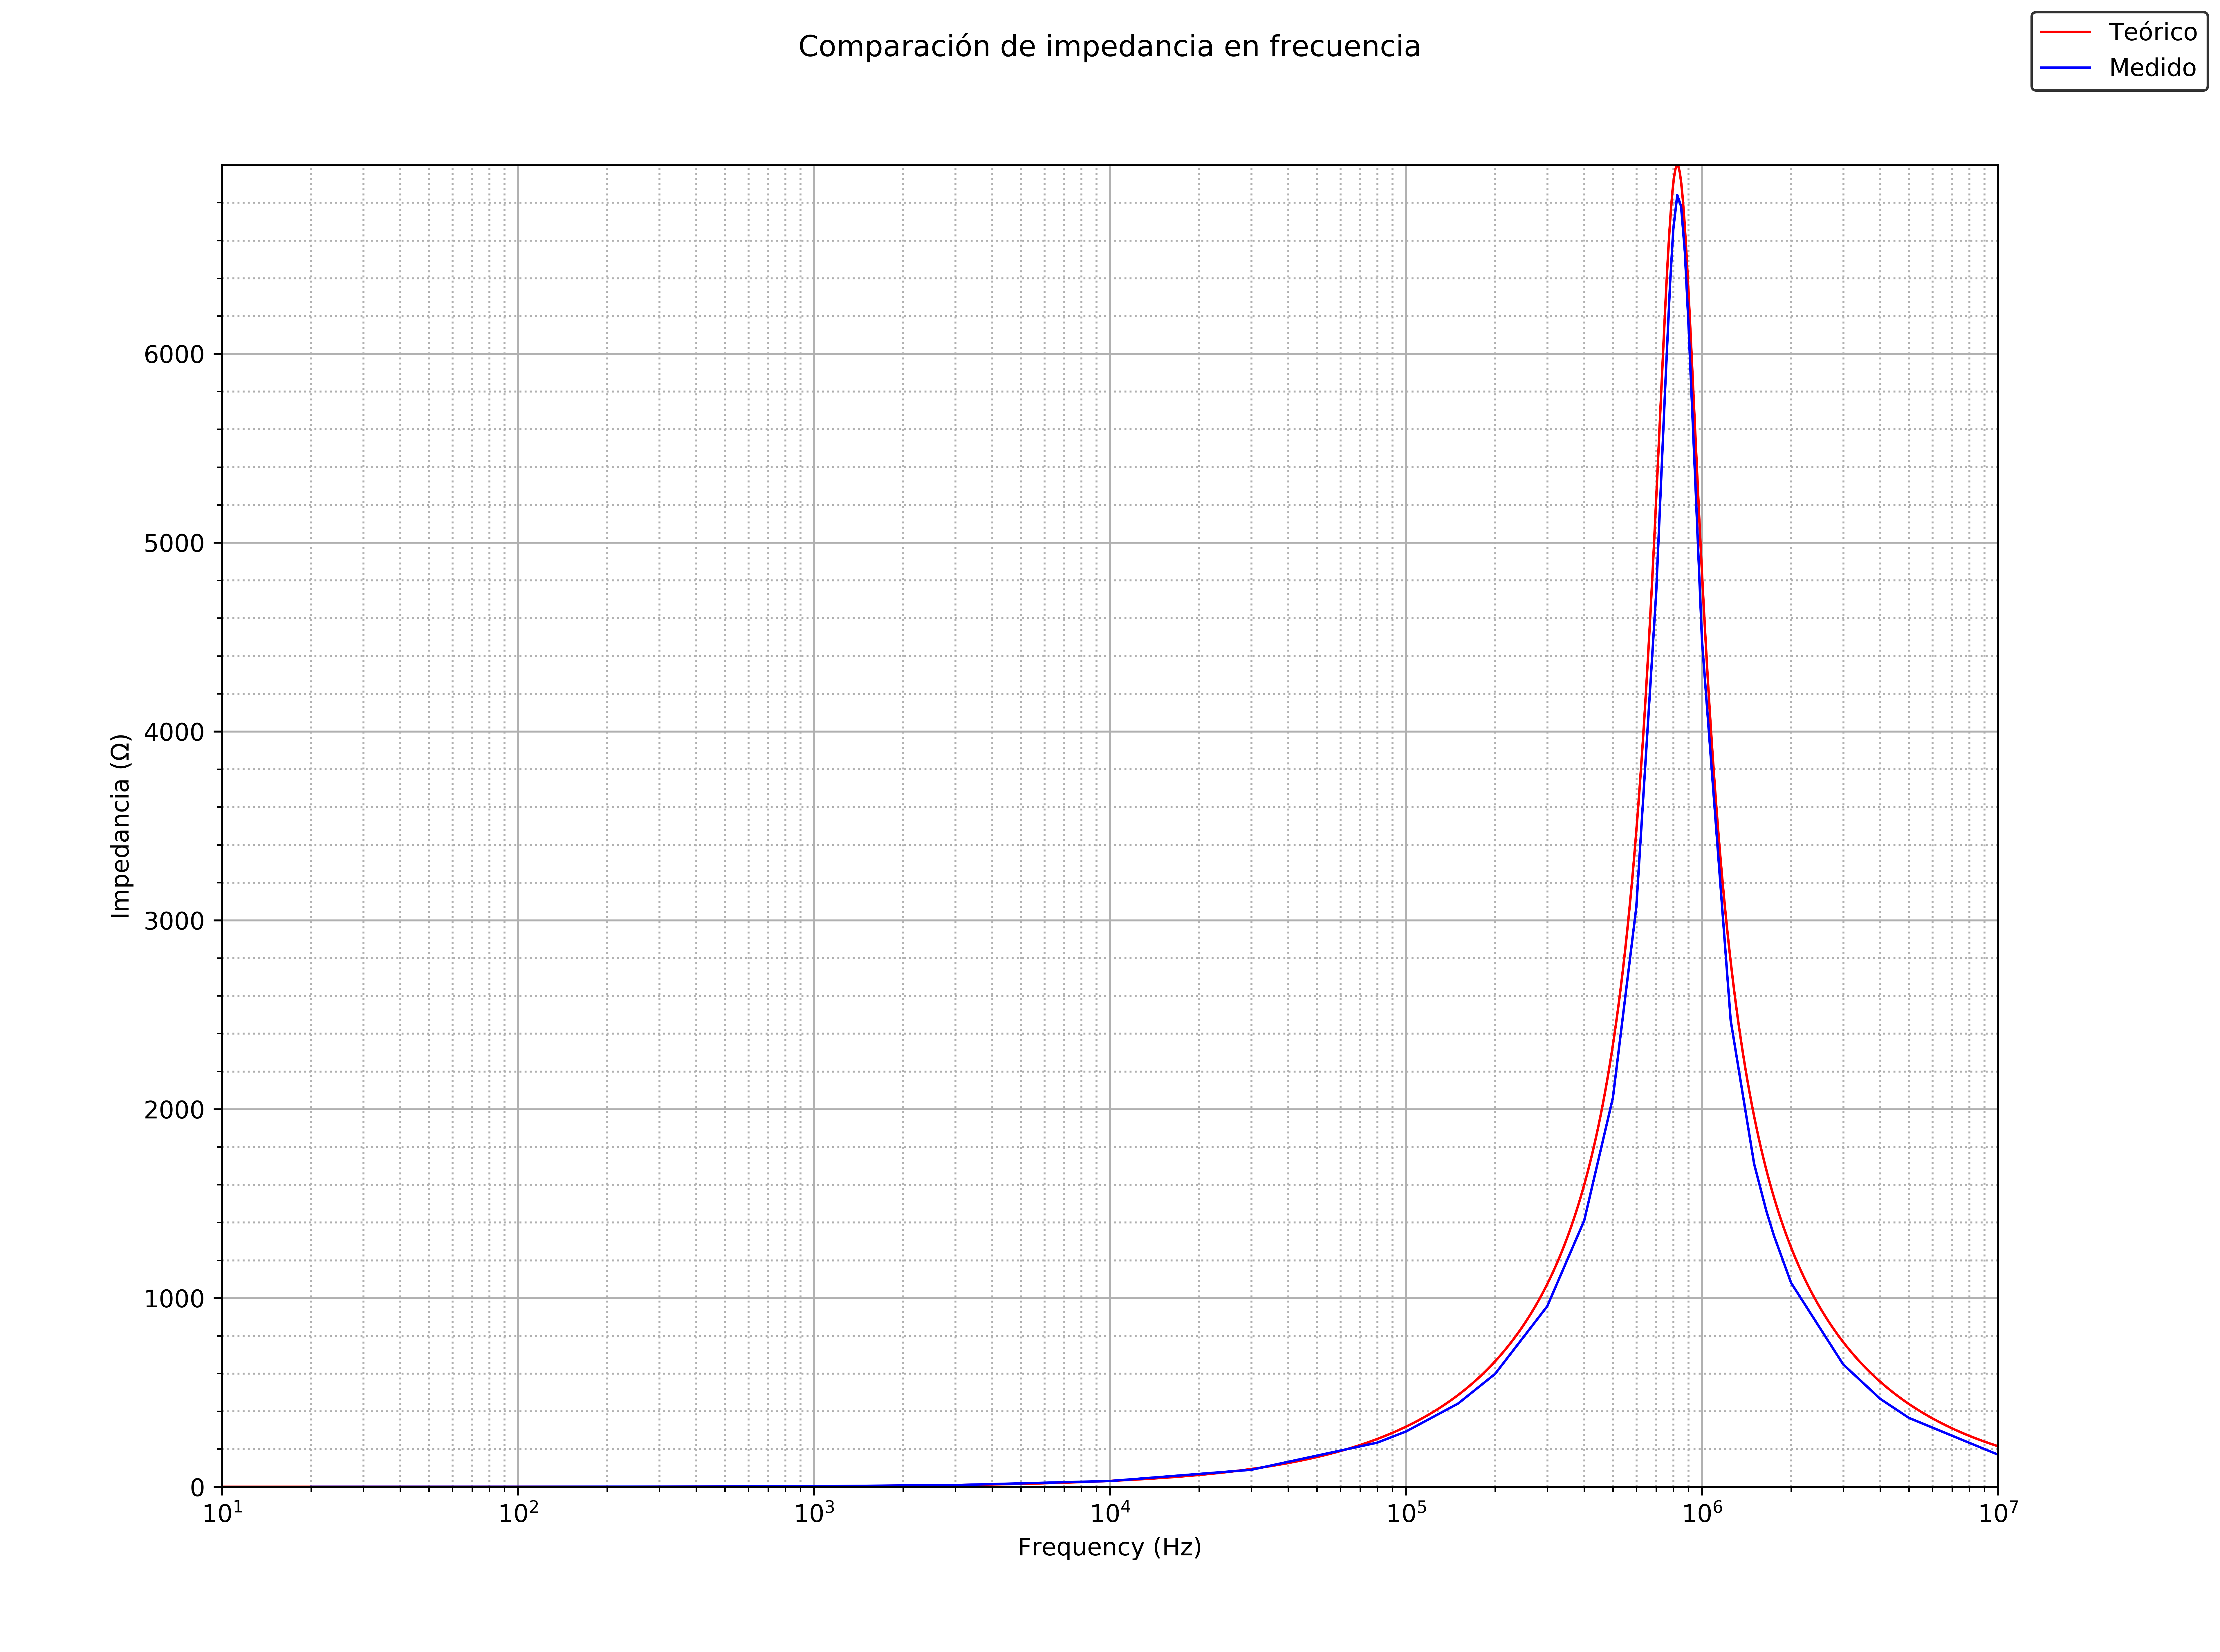
\includegraphics{Recursos/comp_impedancia_ind.png} &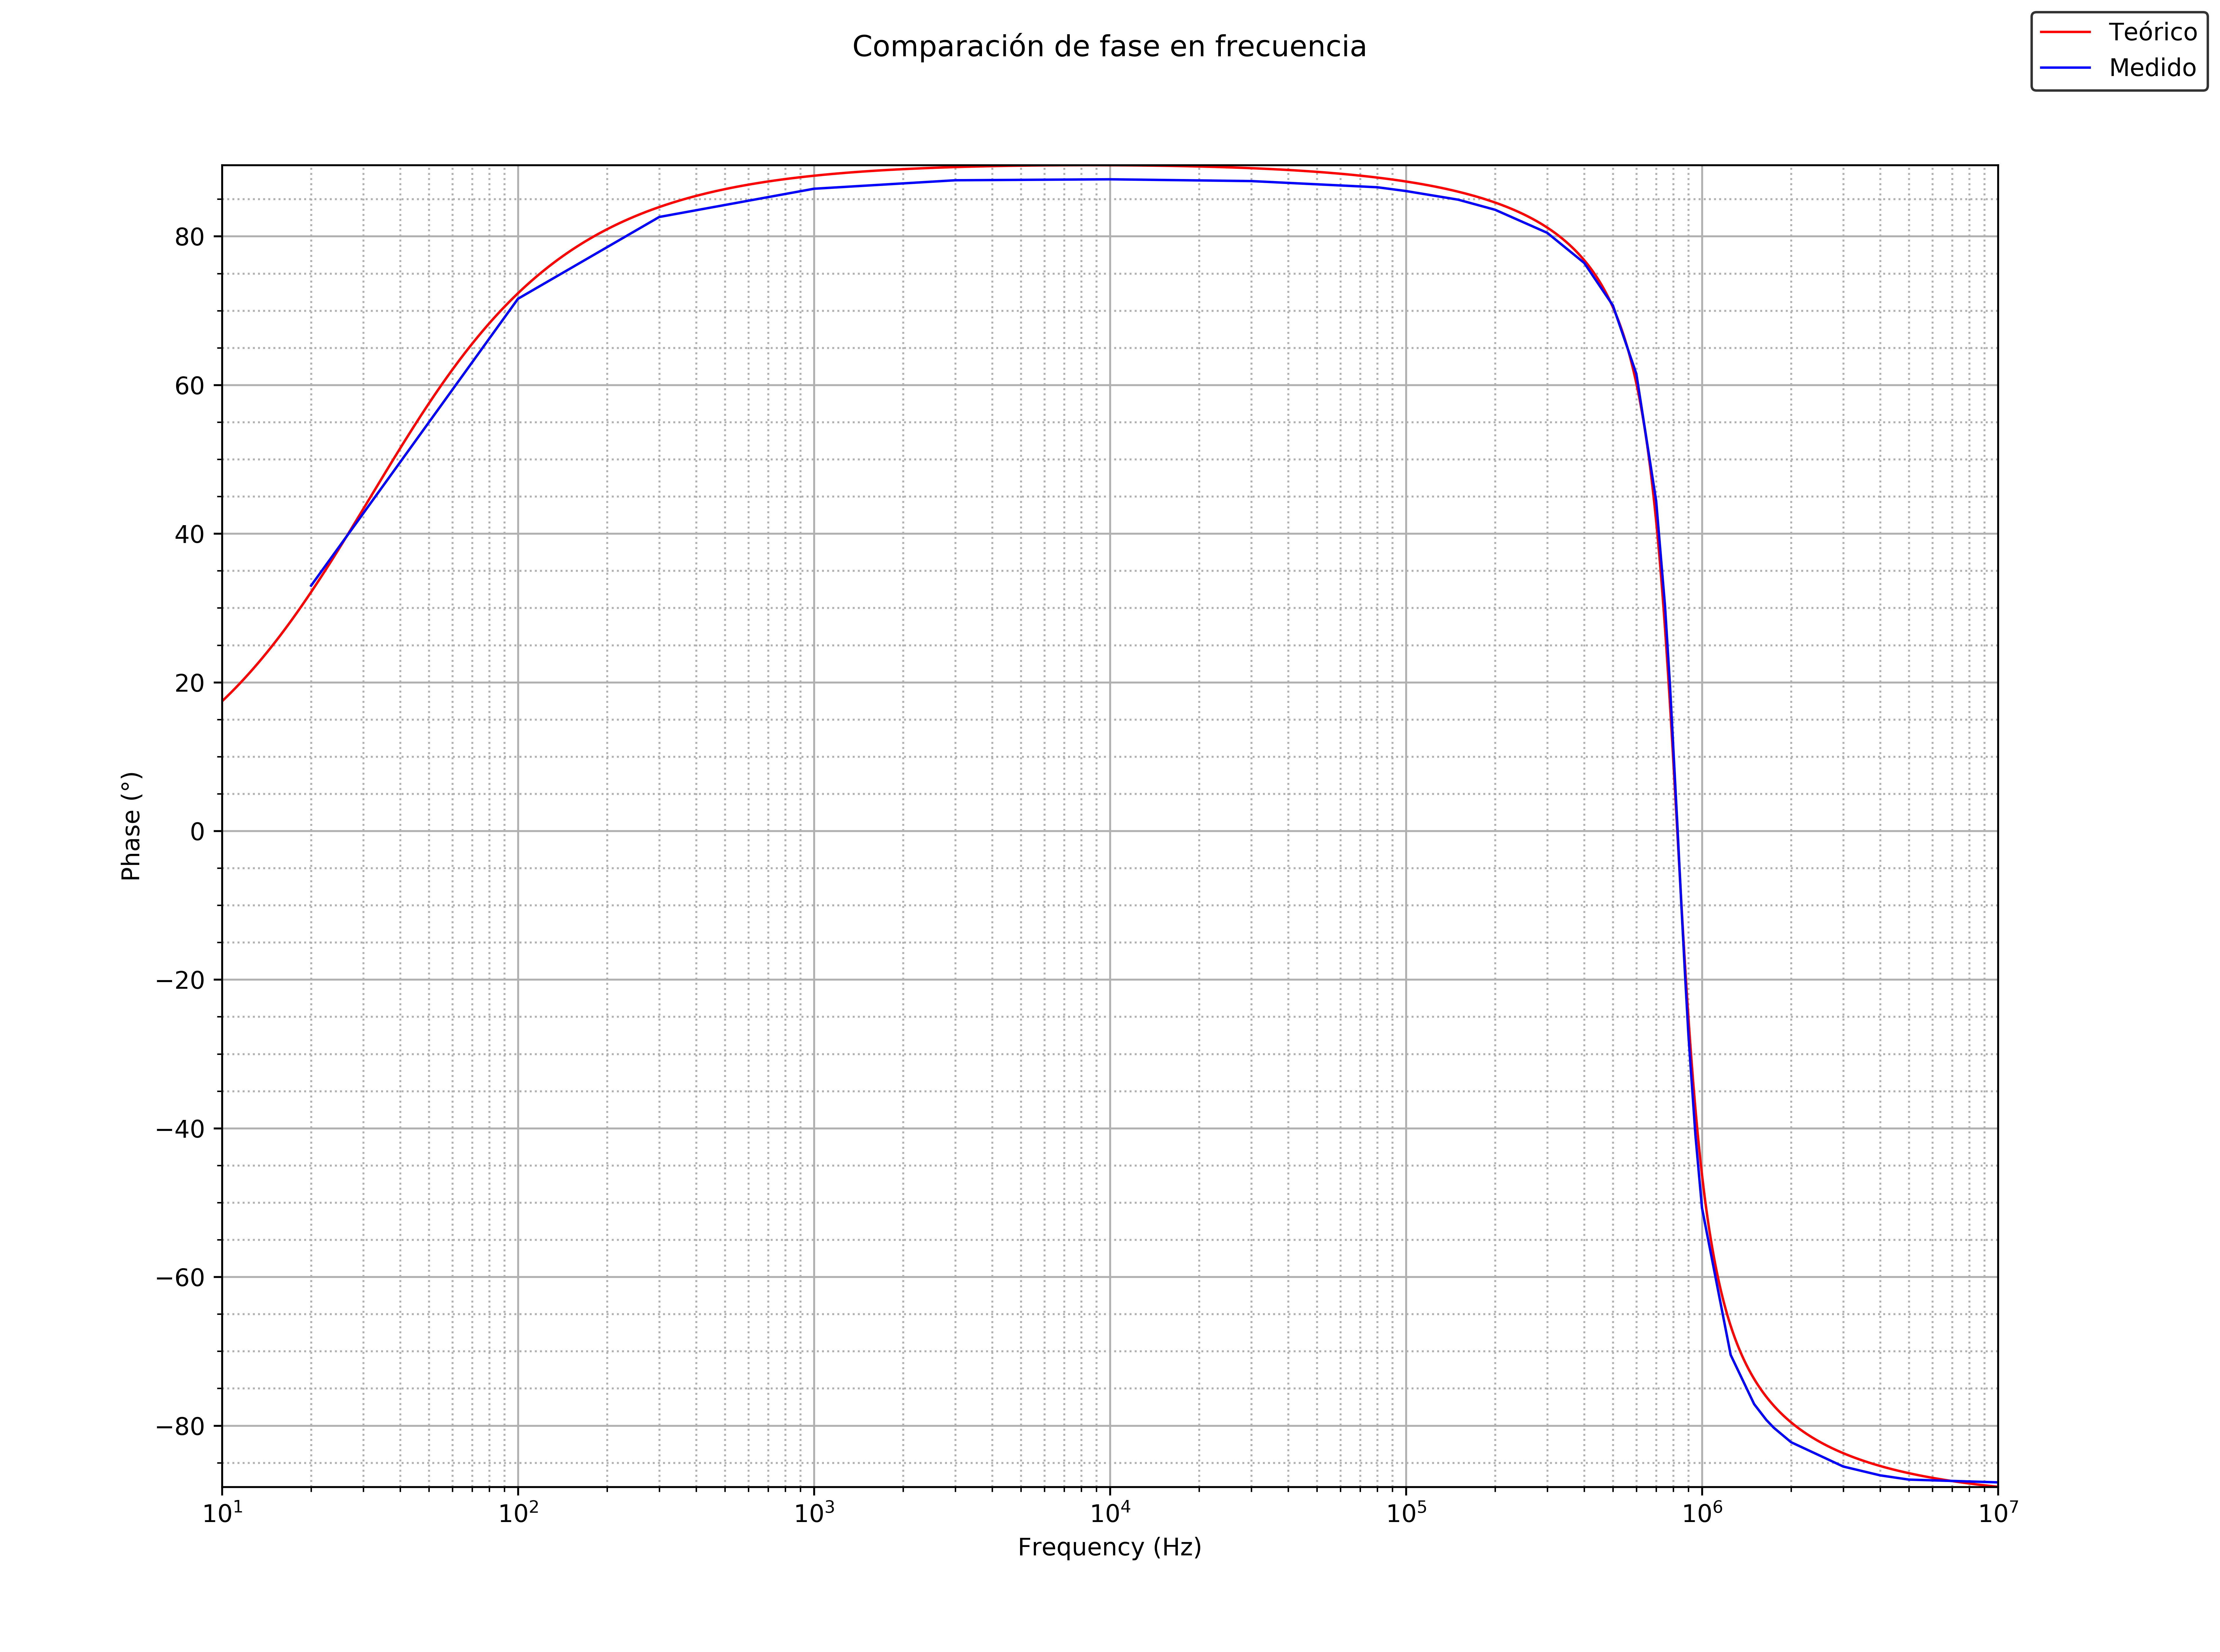
\includegraphics{Recursos/comp_fase_ind.png}
        \end{tabular}
        
    }
    \caption{Comparaci\'on entre mediciones y modelo de impedancia y fase en funci\'on de la frecuencia. }
        \label{fig:Comp_IND}    
\end{figure}

En este caso se observa un ajuste mucho mejor con las curvas medidas.


\subsection{Conclusiones}
Es posible observar en las distintas curvas mostradas en esta secci\'on, las variaciones que los componentes pasivos tienen con la frecuencia. 

Para una frecuencia fuera del rango de operaci\'on, un capacitor puede comportarse como un inductor y viceversa. Es por esto que es de suma importancia, al dise\~nar un circuito de apliaci\'on, elegir correctamente el modelo con el que se trabaja.
    \newpage
    
\section{2. Puente de Wien - Medici\'on de frecuencias}


El puente de Wien es un tipo de puente que consiste en dos capacitores y cuatro resistores. El mismo puede utilizarse para el cálculo de frecuencias lográndose la siguiente condición de balance:


\begin{figure}[H]
\begin{center}
\begin{circuitikz}
	
	\node [](Vg){}; 
	\draw (Vg) to[american voltage source , l = $V_g$] ++(0, -6) to[short] ++(4.5, 0);	
	\draw (Vg) to[short] ++(1.5, 0) node[](begin){} to[C, l =$C_1$] ++(0, -1.5) to[R, l = $R_1$] ++(0, -1.5) node[](vdl){};
	\draw (vdl) to[short] ++(0, -0.5) node[](parallel){};
	\draw (parallel) to[short] ++(1.25,0) to[R, l = $R_3$] ++(0, -2) to[short] ++(-1.25,0);
	\draw (parallel) to[C, l = $C_3$] ++(0, -2) to[short] ++(0, -0.5) node[ground]{};
	
	\draw (begin) to[short] ++(3,0) to[R, l = $R_2$] ++(0, -3) to[R, l = $R_4$] ++(0, -3);
	\draw (vdl) to[short] ++(3,0);
	

\end{circuitikz}
	\caption{Puente de Wien}
	\label{fig:Wien}
\end{center}
\end{figure}

\begin{equation}
f = \frac{1}{2\pi\sqrt{R_1R_3C_1C_3}}
\end{equation}

Para el caso en el que $R_1 = R_3$ y $C_1 = C_3$ la igualdad se simplifica:

\begin{equation}
f = \frac{1}{2\pi RC}
\end{equation}

con $R$ y $C$ el valor de los componentes.


En general se busca ajustar los valores de $R_1$ y $R_3$ para que coincidan y as\'i se cumpla la condici\'on de puente.

Asimismo se debe considerar $R_2 = 2 \cdot R_4$ para que se cumpla dicha condici\'on.

%%agregar aca sensibilidades 
\subsection{Diseno y elecci\'on de componentes}

Los componentes fueron seleccionados realizando c\'alculos para que el puente pueda estabilizarse en el rango de frecuencias solicitado ($100Hz$ a $2KHz$). De esta forma se tiene la siguiente distribuci\'on, tomando en cuenta las suposiciones realizadas con anterioridad.

\begin{table}[H]
    \centering
    \begin{tabular}{c c c c}
        $C_1 = C_3$ & $R_2 = 2 \cdot R_4$ & $R_1 = R_3 (preset)$ \\
        \hline \\
        $33 nF$ & $10 K\Omega$ & $50 K\Omega$ \\
        \hline
    \end{tabular}
\end{table}

Cabe destacar que se consider\'o un cierto margen en el rango de frecuencias, teniendo en cuenta las tolerancias de los componentes.



\subsubsection{Sensibilidades}
Se calcul\'o la sensibilidad del puente respecto a los componentes que se eligi\'o variar ($R_1$ y $R_3$).

La sensibilidad respecto de $R_1$ se puede calcular como:

\begin{equation}
\Delta V_d = \frac{Z_3 \cdot (Z_2+Z_4) - Z_4(Z_1 + \Delta Z_1 + Z_3)}{(Z_1+Z_3) \cdot (Z_2+Z_4)} \cdot v_g
\end{equation}
 
Veamos que

\begin{equation}
\frac{|\Delta Z_1|}{|Z_1|} = \frac{\Delta R_1}{|Z_1|} = \frac{\frac{\Delta R_1}{R_1}}{\sqrt{1+\frac{1}{(\omega \cdot C_1 \cdot R_1)^2}}}
\end{equation}

Suponiendo $\frac{1}{\omega \cdot C_1 \cdot R_1} >> 1$ obtenemos:

\begin{equation}
\frac{|\Delta Z_1|}{Z_1} = \frac{|\Delta R_1|}{R_1} \cdot \omega \cdot C_1 \cdot R_1
\end{equation}


Sabiendo esto, y asumiendo condici\'on de puente y $v_g$ unitario obtenemos

\begin{equation}
\Delta V_d = \frac{-A}{(A+1)^2} \cdot \omega \cdot R_1 \cdot C_1 \cdot \frac{\Delta R_1}{R_1}
\end{equation}

Donde $A = \frac{R_2}{R_4}$ es el factor cabeza de puente, y esta relaci\'on fue fijada con anterioridad. 

Asumiendo los valores de la tabla de selecci\'on de componentes, se grafica la sensibilidad para el rango de frecuencia.

\begin{figure}[H]
    \centering
    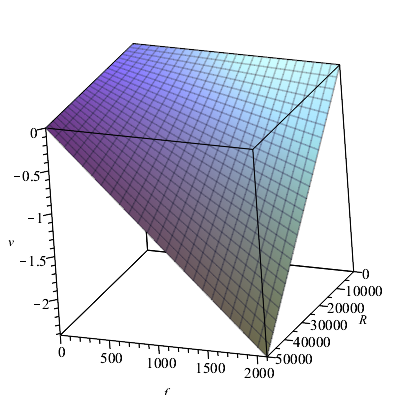
\includegraphics[width=0.9\textwidth]{Recursos/sensib_R1.png}
	\caption{Sensibilidad del circuito respecto a $R_1$}
   	\label{fig:sensib_R1}
\end{figure}

Se realiza un procedimiento an\'alogo para obtener la sensibilidad del puente respecto a $R_3$.

Veamos que:

\begin{equation}
Z_3 + \Delta Z_3 = \frac{R_3 + \Delta R_3}{1+S \cdot C_3 \cdot (R_3 + \Delta R_3)} 
\end{equation}

Suponemos $R_3 >> \Delta R_3$ y despreciamos los efectos de $\Delta R_3$ sobre el denominador debido a que est\'a multiplicado por un n\'umero relativamente peque\~no para el rango de frecuencias.

Luego se tiene

\begin{equation}
Z_3 + \Delta Z_3 = \frac{R_3}{1+S \cdot C_3 \cdot R_3} + \frac{\Delta R_3}{1+S \cdot C_3 \cdot R_3} = Z_3 + \frac{\Delta R_3}{1+S \cdot C_3 \cdot R_3}.
\end{equation}

Por lo que $\Delta Z_3 = \frac{\Delta R_3}{1+S \cdot C_3 \cdot R_3}$

Operando, se llega a la siguiente equivalencia:

\begin{equation}
\frac{|\Delta Z_3|}{|Z_3|} = \frac{\Delta R_3}{R_3}
\end{equation}

Finalmente, considerando $V_g$ unitario,

\begin{equation}
\Delta V_d = \frac{A}{(A+1)^2} \cdot \frac{\Delta R_3}{R_3}
\end{equation}

Por lo que ser\'a constante independientemente de la frecuencia ($V_d = \frac{2}{9}$).


\subsection{Mediciones}

Para la medici\'on del puente se utiliz\'o el mult\'imetro de banco. Con el mismo es posible medir niveles de tensi\'on que ser\'ian indistinguibles del ruido en un osciloscopio. Se estimul\'o al circuito con una senal de $5V_{pp}$ y se ajustaron los dos potensi\'ometros hasta obtener la menor tensi\'on posible:


\begin{table}[H]
\centering
\begin{tabular}{lllll}
Frecuencia del generador & Preset R\_1(Ohm) & Preset R\_2(Ohm) & Frecuencia calculada & Error(\%) \\ \hline
100                      & 46100            & 45915             & 104.83              & 3,92      \\
500                      & 9390             & 9175             & 519,6             & 4,83      \\
750                      & 6283             & 6219             & 771,55               & 2,87      \\
1000                     & 4695             & 4689             & 1027,89              & 2,79      \\
1250                     & 3833             & 3762             & 1270                 & 1,61      \\
1500                     & 3144             & 3125             & 1538,65              & 2,58      \\
1750                     & 2704             & 2665             & 1795,6               & 2,66      \\
2000                     & 2331             & 2318             & 2074,8               & 3,74     \\ \hline
\end{tabular}
\end{table}

En primer lugar se observa el comportamiento esperado respecto a las resistencias, para medir una frecuencia más cercana al límite inferior de la escala propuesta se precisan resistencias mayores. Además de lo anterior es importante hacer notar que el balance se logra solamente cuando ambos potenciómetros poseen resistencias casi iguales. Este balance no fue ideal, ya que no pudo llegarse a una diferencia de potencial igual a 0 entre ambas ramas, en cambio se tomó como $0$ el menor valor posible dada la frecuencia medida. Dicha tensión fue siempre menor a $10mV$. Dado el voltaje con el que se estimuló al circuito y el error porcentual obtenido  puede cdecirse que los resultados son satisfactorios y queda poco lugar para mejoras. Incluir las resistencias equivalentes de los capacitores utilizados tanto como las capacitancias parásitas de las resistencias es una de esas mejoras. No obstante, dadas las frecuencias en las que se trabajó, las capacitancias y las resistencias parásitas son despreciables en comparación a las tolerancias reales de los componentes. 




\subsection{Conclusiones}

Como conclusi\'on se puede destacar que se notaron diferencias entre el modelo te\'orico del puente y las mediciones realizadas en la pr\'actica. Principalmente se observa que es muy dificil equilibrar el puente en su totalidad, debido a las variaciones en los presets de ajuste y las tolerancias asociadas a los componentes del circuito.
    \newpage
    
\section{3. Puente de medici\'on de capacitores}
El objetivo de esta secci\'on es realizar el an\'alisis y dise\~no de un circuito puente denominado C Serie, con el fin de poder medir diferentes tipos de capacitores de prueba, tanto su par\'ametro de capacidad como factor de p\'erdidas del mismo.

\begin{figure}[H]
    \centering
    \includegraphics[scale=0.7]{Recursos/cserie.png}
    \caption{Puente C Serie}
    \label{fig:puente_c_serie}
\end{figure}

\subsection{An\'alisis te\'orico}
Se propone establecer un valor fijo para el capacitor patr\'on $C_1$ y la resistencia $R_4$, as\'i se utilizan $R_3$ y $R_1$ como variables de ajuste para llevar al puente a la condici\'on de equilibrio, para lo cual se definir\'a en cada caso un valor m\'inimo y m\'aximo seg\'un los rangos de operaci\'on del puente de medici\'on. 
Vale mencionar que para implementar el rango de variaci\'on de las variables de ajuste, se har\'a uso de una resistencia en serie junto con presets o trimmers de diferentes valores para garantizar tanto un ajuste grueso como fino del puente.

\subsubsection{Condiciones de dise\~no}
Se desea dise\~nar un puente de medici\'on C Serie que opere a una frecuencia de $f = 20kHz$. Debe ser capaz de medir capacitores que se encuentren dentro del rango $10nF < C < 100nF$ y $0.02 < D < 0.12$.

\subsubsection{Ecuaciones del puente}
\begin{equation}
\begin{array}{lllll}
    \frac{V_d}{V_g} = \frac{Z_3\cdot Z_x - Z_4 \cdot Z_1}{Z_1 \cdot Z_x + Z_1 \cdot Z_4 + Z_3\cdot Z_x + Z_3 \cdot Z_4}\\
    Z_1 = \frac{1}{s\cdot C_1} + R_1\\
    Z_x = \frac{1}{s\cdot C_x} + R_x\\
    Z_3 = R_3\\
    Z_4 = R_4\\
\label{eq:Ec_puente}
\end{array}
\end{equation}

\subsubsection{Sensibilidades del puente}
El proceso de medici\'on de un puente requiere alcanzar la condici\'on de equilibrio a trav\'es del ajuste de sus diversas variables, para lo cual es de inter\'es conocer con qu\'e sensibilidad var\'ia la condici\'on respecto de los cambios en tales variables. Para este an\'alisis se emplea la definici\'on de sensibilidad absoluta, asumiendo cambios o variaciones no muy grande se hace un c\'alculo en diferencias de las variables.

\paragraph{Sensibilidad respecto de la variable $Z_3$}

\begin{equation}
    V_d + \Delta V_d=\frac{(Z_3+ \Delta Z_3)\cdot Z_x - Z_4 \cdot Z_1}{Z_1 \cdot Z_x + Z_1 \cdot Z_4 + (Z_3+ \Delta Z_3)\cdot Z_x +(Z_3+ \Delta Z_3) \cdot Z_4} \cdot V_g
    \label{eq:Sensibilidad_Z3_1}
\end{equation}

\begin{equation}
     Z_3 \gg \Delta Z_3 \Rightarrow
    \Delta V_d = \frac{\frac{\Delta Z_3}{Z_3}}{\left(\frac{Z_1}{Z_3}+ 1\right)\left(\frac{Z_4}{Z_x} + 1\right)} \cdot V_g
\end{equation}

Se define, asumiendo que se cumple la condici\'on de puente balanceado, $A=\frac{Z_1}{Z_3}=\frac{Z_x}{Z_4}$.

\begin{equation}
\Delta V_d = \frac{A}{(A+1)^2} \cdot \frac{\Delta Z_3}{Z_3} \cdot V_g = \frac{A}{(A+1)^2} \cdot \frac{\Delta R_3}{R_3} \cdot V_g 
\label{eq:sens_z3_cabezapuente}
\end{equation}

\paragraph{Sensibilidad respecto de la variable $Z_1$}

\begin{equation}
    \Delta V_d = - \frac{\frac{\Delta Z_1}{Z_1}}{\left(\frac{Z_3}{Z_1}+ 1\right)\left(\frac{Z_x}{Z_4} + 1\right)} \cdot V_g
\end{equation}

 \begin{equation}
    \left| \frac{\Delta Z_1}{Z_1} \right| = \frac{\Delta R_1}{|Z_1|} = \frac{\frac{\Delta R_1}{R_1}}{\sqrt{1 + \left(\frac{1}{\omega \cdot C_1 \cdot R_1 }\right)^2}}
\end{equation}

\begin{equation}
    \frac{1}{\omega \cdot C_1 \cdot R_1 }\gg 1 \Rightarrow
    \left| \frac{\Delta Z_1}{Z_1} \right| = \frac{\Delta R_1}{R_1}\cdot\omega \cdot C_1 \cdot R_1 
\end{equation}

\begin{equation}
   \Delta V_d = - \frac{\frac{\Delta R_1}{R_1}\cdot\omega \cdot C_1 \cdot R_1 }{\left(\frac{Z_3}{Z_1}+ 1\right)\left(\frac{Z_x}{Z_4} + 1\right)} \cdot V_g
\end{equation}

\begin{equation}
   \Delta V_d = \frac{A}{(A+1)^2}\cdot \frac{\Delta Z_1}{Z_1}\cdot\omega \cdot C_1 \cdot R_1 \cdot V_g
\end{equation}

\subsubsection{Dimensionamiento del puente}
Se obtienen de la condici\'on de puente balanceado, las ecuaciones que se muestran en \ref{eq:D_C_R_x}. A partir de estas, y de las condiciones sobre los m\'aximos valores medibles de capacidad y factor de p\'erdidas que se observan en la Tabla \ref{tab:condiciones_de_diseno}, se obtienen valores l\'imite para los presets a utilizar al realizar la medici\'on.
\begin{equation}
    \centering
        \begin{array}{ccc}
            C_x = \frac{C_1\cdot R_3}{R_4}\\
            R_x = \frac{R_1 \cdot R_4}{R_3}\\
            D_x = \omega\cdot C_1 \cdot R_1
            
        \end{array} 
    \label{eq:D_C_R_x}
\end{equation}
\begin{table}[H]
\centering
\resizebox{0.4\textwidth}{!}{%
\begin{tabular}{ccl}
\hline
Par\'ametros & M\'inimo & M\'aximo \\ \hline
$C_x$ & 10nF & 100nF \\
$D_x $& 0.02 & 0.12 \\
f & \multicolumn{2}{c}{20KHz} \\ \hline
\end{tabular}%
}
\caption{Condiciones de dise\~no del puente}
\label{tab:condiciones_de_diseno}
\end{table}

Se fijan valores para $C_1$ y $R_4$ de $1nF$ y $100\Omega$ respectivamente. A partir de estos valores se obtiene un rango posible para $R_3$ y $R_1$ que permiten lograr el equilibrio en cualquier caso donde se cumplan las condiciones impuestas. Se muestran en la Tabla \ref{table:Rangos_pot}, los resultados de dicho an\'alisis. 

\begin{table}[H]
\centering
\begin{tabular}{ccc}
\hline
Resistencias & M\'inimo & M\'aximo \\ \hline
$R_1$ & $159.15 \Omega$ & $954.9 \Omega$ \\
$R_3 $& $1 k\Omega$ & $10 k\Omega$ \\
\end{tabular}
\caption{Rango de valores }
\label{table:Rangos_pot}
\end{table}

Finalmente, se propone utilizar una resistencia $R_1$ compuesta por el conjunto serie de una resistencia de $R = 150 \Omega$ en serie con dos presets, uno de $1k\Omega$ y uno de $100\Omega$ de forma tal que la precisi\'on del cambio pueda ajustarse con mayor o menor paso. De igual forma en $R_3$ con una resistencia de $1k \Omega$ y dos presets de $10k\Omega$ y $1k \Omega$.

\begin{figure}[H]
    \centering
    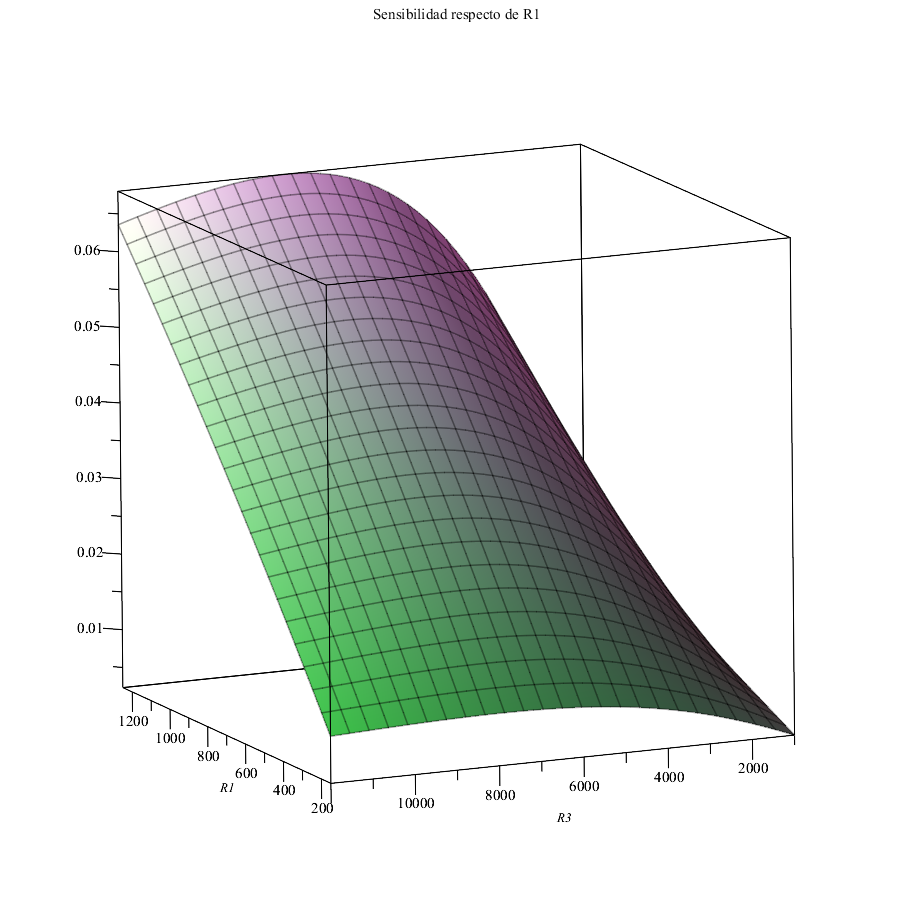
\includegraphics[scale=0.4]{Recursos/cserie_sensibilidad_r1.png}
    \caption{Sensibilidad respecto de R1}
    \label{fig:sensibilidad_r1}
\end{figure}

\begin{figure}[H]
    \centering
    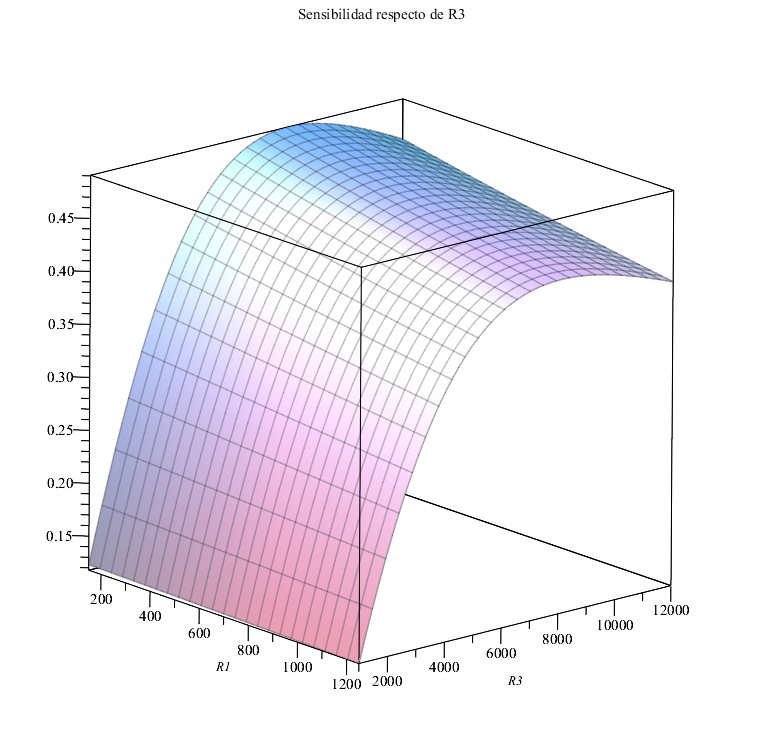
\includegraphics[scale=0.4]{Recursos/cserie_sensibilidad_r3.png}
    \caption{Sensibilidad respecto de R3}
    \label{fig:sensibilidad_r3}
\end{figure}

\begin{figure}[H]
    \centering
    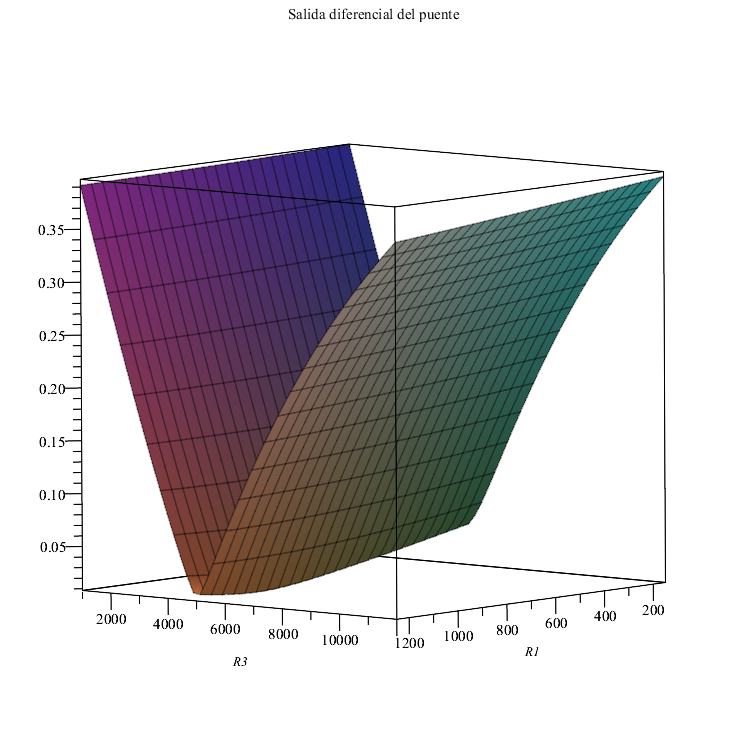
\includegraphics[scale=0.4]{Recursos/cserie_salida.png}
    \caption{Salida del puente variando R1 y R3}
    \label{fig:salida_puente_cserie}
\end{figure}



\subsection{Resultados}

\subsubsection{Componentes patr\'on}
Se emplea un analizador de impedancias para medir los componentes patr\'on utilizados en la implementaci\'on f\'isica del circuito puente. En ambos casos sea realiza la medici\'on con una frecuencia de  $f = 2kHz$, $f = 20kHz$ y $f = 200kHz$

\begin{table}[H]
    \centering
    \begin{tabular}{c c c c}
        $f [Hz]$ & $R [\Omega]$ & $C [F]$ & $D$ \\
        \hline \\
        $2kHz$ & $98.68\Omega$ & $955pF$ & $0.088$ \\
        $20kHz$ & $98.68\Omega$ & $938pF$ & $0.098$ \\
        $20kHz$ & $98.68\Omega$ & $926pF$ & $0.0145$ \\
        \hline
    \end{tabular}
    \caption{Componentes patr\'on del puente}
    \label{tab:mediciones_componentes_patron}
\end{table}

\subsubsection{Mediciones del puente}
Se utilizan diferentes capacitores arbitrarios como elementos de prueba del proceso de medici\'on empleando el puente dise\~nado. Se realizan las mediciones para las frecuencias de $f = 2kHz$, $f = 20kHz$ y $f = 200kHz$.

\begin{table}[H]
    \centering
    \begin{tabular}{c | c c c  c c c  c c c}
         Valor Nominal & \multicolumn{3}{c}{$f = 2kHz$} & \multicolumn{3}{c}{$f = 20kHz$} & \multicolumn{3}{c}{$f = 200kHz$} \\
         & $C$ & $D$ & $\phi$ & $C$ & $D$ & $\phi$ & $C$ & $D$ & $\phi$  \\
         \hline \\
         $10nF$ & $12.5nF$ &0.016 &$-89.05^\circ$& $9.79nF$&0.16&$-80.76^\circ$ &$9.29nF$ &1.64 &$-31.37^\circ$ \\
         $47nF$ & $43.9nF$&0.016 & $-89.03^\circ$& $48.1nF$&0.087 &  $-85.01^\circ$& $45.5nF$& 0.173&$-80.16^\circ$  \\
         $100nF$ & $105nF$& 0.006& $-89.62^\circ$& $105nF$ &0.025 &$-88.51^\circ$ &$107nF$ & 0.256&$-75.64^\circ$  \\
         $220nF$ &$107nF$ &0.003 & $-89.77^\circ$&$105nF$ & 0.033& $-88.1^\circ$&$104nF$ & 0.173& $-80.16^\circ$ \\
         \hline
    \end{tabular}
    \caption{Mediciones del puente}
    \label{tab:mediciones_del_puente}
\end{table}

\subsubsection{Mediciones del analizador de impedancias}
Se utiliza el analizador de impedancia para medir los mismos componentes arbitrarios que fueron medidos con el puente para realizar una apreciaci\'on de las diferencias. Se realizan las mediciones para las frecuencias de $f = 2kHz$, $f = 20kHz$ y $f = 200kHz$.

\begin{table}[H]
    \centering
    \begin{tabular}{c | c c c  c c c  c c c}
         Valor Nominal & \multicolumn{3}{c}{$f = 2kHz$} & \multicolumn{3}{c}{$f = 20kHz$} & \multicolumn{3}{c}{$f = 200kHz$} \\
         & $C$ & $D$ & $\phi$ & $C$ & $D$ & $\phi$ & $C$ & $D$ & $\phi$  \\
         \hline \\
         $10nF$ & $9.57nF$ &0.856 &$-49.3^\circ$& $9.57nF$&0.097&$-84.4^\circ$ &$9.28nF$ &0.024 &$-88.58^\circ$ \\
         $47nF$ & $47.3nF$&0.174 & $-80.12^\circ$& $46.8nF$&0.027 &  $-88.45^\circ$& $46.1nF$& 0.023&$-88.63^\circ$  \\
         $100nF$ & $107nF$& 0.507& $-63.05^\circ$& $106nF$ &0.061 &$-86.42^\circ$ &$104nF$ & 0.025&$-88.59^\circ$  \\
         $220nF$ &$200nF$ &0.035 & $-87.92^\circ$&$180nF$ & 0.032& $-88.13^\circ$&$162nF$ & 0.029& $-88.34^\circ$ \\
         \hline
    \end{tabular}
    \caption{Mediciones del puente}
    \label{tab:mediciones_del_puente}
\end{table}

\subsection{Manual de usuario}

En la Fig. \ref{fig:circuito_puente_final} se muestra un esquema general del circuito puente dise\~nado en el cual se puede apreciar que las variables de ajuste son $R_1$ y $R_3$, utilizando tanto un preset de ajuste fino como grueso para ambos casos. Se dispone de una entrada y una salida al mismo, el objetivo del proceso de medici\'on es aplicar una se\~nal de entrada dada y medir la salida diferencial, variando el ajuste hasta alcanzar el equilibrio en el cual $V_d = 0$. Finalmente se usan el conjunto de ecuaciones \ref{eq:D_C_R_x} para obtener los resultados.

\begin{figure}[H]
    \centering
    \includegraphics[scale=0.4]{Recursos/puente.png}
    \caption{Esquema general del circuito dise\~nado}
    \label{fig:circuito_puente_final}
\end{figure}

En la Fig. \ref{fig:conexion_puente} se ilustra un esquema general de la conexi\'on del puente. Se debe utilizar un generador de funciones o se\~nales configurando el mismo con una senoidal de un valor de amplitud $V_G = 1 V_{PP}$ con la frecuencia a la cual se desea analizar el capacitor. Finalmente, se emplea un osciloscopio con dos canales para medir ambas salidas del dispositivo y utilizando la funcionalidad Math calcular la diferencia entre ellas, variando el ajuste hasta alcanzar el equilibrio del puente.

\begin{figure}[H]
    \centering
    \includegraphics[scale=0.5]{Recursos/manual_cserie.png}
    \caption{Esquema de conexi\'on}
    \label{fig:conexion_puente}
\end{figure}

\begin{table}[H]
    \centering
    \begin{tabular}{c | c c c}
        Magnitud & M\'in. & \'Optimo & M\'ax. \\
        \hline \\
        $f$ & $2kHz$ & $20kHz$ & $2kHz$ \\
        $V_G$ & $-$ & $1 V_{PP}$ & $-$ \\
        $R_1$ & $150 \Omega$ & $-$ & $1250 \Omega$ \\
        $R_3$ & $1k \Omega$ & $-$ & $12k \Omega$ \\
        $C_x$ & $10nF$ & $-$ & $100nF$ \\
        $D_x$ & $0.02$ & $-$ & $0.12$ \\
        \hline
    \end{tabular}
    \caption{Especificaciones}
    \label{tab:especificaciones}
\end{table}

\subsection{Precisi\'on del puente}
Se calcula, tomando las mediciones realizadas con el analizador de impedancias como valor real, el error relativo porcentual cometido en las mediciones. Esto permite tener una idea de la precis\'on del puente y en error cometido al medir.

Se calcula el error relativo como $E_{\%Rel} = \frac{Valor_{medido}-Valor_{real} }{Valor_{real}}\cdot 100$. Al hacer este calculo para todas las mediciones realizadas se obtiene la Tabla \ref{tab:TAB_ERROR}
\begin{table}[H]
    \centering
    \resizebox{0.4\textwidth}{!}{%
    \begin{tabular}{cccc}
     & Frecuencia (Hz) & $E_{Cx}$ & $E_{Dx}$ \\ \hline
     \multirow{3}{*}{10nF} & 2000 & 30.45\% & 98.07\% \\
     & 20000 & $2.31\%$ & $66.66\%$ \\
     & 200000 & $0.11\%$ & $6511.20\%$\\ \hline
    \multirow{3}{*}{47nF} & 2000 & $7.05\%$ & $90.31\%$ \\
     & 20000 & $2.77\%$ & $221.87\%$ \\
     & 200000 & $1.21\% $& $625.45\%$ \\ \hline
    \multirow{3}{*}{100nF} & 2000 & $1.51\%$ &$ 98.70\%$ \\
     & 20000 & $0.92\%$ & $58.04\% $\\
     & 200000 & $2.86\%$ & $924.01\%$ \\ \hline
    \multirow{3}{*}{220nF} & 2000 & $46.66\% $& $89.24\%$ \\
     & 20000 & $41.54\%$ & $2.55\%$ \\
     & 200000 & $35.99\%$ & $497.87\%$ \\ \hline
    \end{tabular}%
    }
    \caption{Error relativo de C y D medidos}
    \label{tab:TAB_ERROR}
    \end{table}

\subsection{Conclusi\'on}
Se puede observar que en cuanto a las mediciones de capacidad a 20KHz y cumpliendo con las condiciones de dise\~no originales, se ajustan muy bien a lo medido con el analizador de impedancias. Se observa un error m\'aximo de aproximadamente 3\%, que se encuentra en un rango correcto de error. 

Para 2KHz y 200KHz se observa un error mayor, sin embargo las mediciones siguen dentro de un rango bajo de error en la mayor\'ia de los casos. Se observa que el error m\'aximo cometido en estas condiciones es del 30.45\%, pero en promedio el error es del 7.2\%.

Para valores de capacidad por fuera de los rangos de dise\~no se observa un error mucho mayor, que se corresponde con lo esperado.

Por \'ultimo, se puede observar que las mediciones del factor de p\'erdidas incurre en un error muy grande. Se asume que esto se debe a un error en el dise\~no del puente sumado a un error de apreciaci\'on cometido al utilizar el osciloscopio para realizar las mediciones. 

\end{document}
